\chapter{Lab 3.1 — K-Means Image Segmentation}
\label{ch:lab31}

\section{Problem Definition}

\begin{problembox}
Apply K-Means clustering to \textbf{pixel color quantization}: reduce an RGB photograph from tens of thousands of unique colors to \textbf{K representative centroids}. This is the same algorithm underlying JPEG compression, artistic palette extraction, and automated object isolation. Evaluate K $\in \{2, 3, 5, 8\}$; select the K that best balances visual fidelity and compression.
\end{problembox}

\subsection{Dataset}
\begin{itemize}
  \item \textbf{Input:} Three RGB photographs. The primary image (\texttt{picture.jpg}) has original resolution $2560\times1920$, resized to $262\times350 = 91{,}700$ pixels. The auxiliary images are \texttt{picture\_2.jpg} ($3648\times5472$, resized to $233\times350 = 81{,}550$ pixels) and \texttt{picture\_3.jpg} ($736\times736$, resized to $350\times350 = 122{,}500$ pixels). If any image is absent, a deterministic landscape is synthesized.
  \item \textbf{Feature space:} Each pixel is a point in $\mathbb{R}^3$ with (R, G, B) channels $\in [0, 255]$.
\end{itemize}

\section{Complete Workflow}

\subsection{Setup and Reproducibility}
The random seed (42) guarantees identical centroid initialization across runs. Five custom modules — \texttt{utils}, \texttt{image\_io}, \texttt{kmeans}, \texttt{visualization}, \texttt{run\_pipeline} — are imported from \texttt{src/}. Output directories are created: \texttt{data/raw/} (source images), \texttt{data/processed/} (resized and segmented artifacts), \texttt{reports/figures/} (all plots).

\subsection{Load the Image}
Three image filenames are iterated. For each image, a summary prints: shape, dtype, pixel intensity range, and \textbf{unique RGB color count} — the baseline for measuring compression ratio. The primary image contains 47{,}119 unique colors; \texttt{picture\_2.jpg} and \texttt{picture\_3.jpg} contain 8{,}231 and 25{,}290 respectively. A healthy photograph at 350px width typically yields 3{,}000--50{,}000 unique colors. The displayed image confirms the file loaded correctly.

\begin{figure}[H]\centering
\begin{figure}[H]
  \centering
  \includegraphics[width=\textwidth]{figures/lab31/original_picture.png}
  \caption{Original Picture 1}
\end{figure}
\begin{figure}[H]
  \centering
  \includegraphics[width=\textwidth]{figures/lab31/original_picture_2.png}
  \caption{Original Picture 2}
\end{figure}
\begin{figure}[H]
  \centering
  
\includegraphics[width=\textwidth]{figures/lab31/original_picture_3.png}
  \caption{Original Picture 3}
\end{figure}
\end{figure}

\begin{figure}[H]\centering
\includegraphics[width=0.7\textwidth]{figures/lab31/original_image.png}
\caption{Primary image loaded for K-Means pixel clustering.}
\end{figure}

\subsection{Preprocess the Image}
\begin{enumerate}
  \item \textbf{Resize:} Max dimension capped at 350px — an uncompressed 4000$\times$3000 image (12M points) is computationally prohibitive. 350px bounds pixels to $\sim$122{,}500, large enough to preserve spatial structure but fast enough for clustering in seconds.
  \item \textbf{Flatten:} \texttt{flatten\_pixels()} reshapes $(H, W, C) \rightarrow (H\!\times\!W, C)$ — the canonical input for vectorized distance computations.
  \item \textbf{Color space preview:} The image is rendered in RGB, HSV, and LAB for visual comparison. \textbf{RGB} clusters raw channel co-occurrence; \textbf{HSV} separates chromatic content (hue) from intensity (value); \textbf{LAB} approximates human perceptual distance — Euclidean proximity in LAB correlates more closely with visible color difference.
\end{enumerate}

\begin{figure}[H]\centering
\begin{figure}[H]
  \centering
  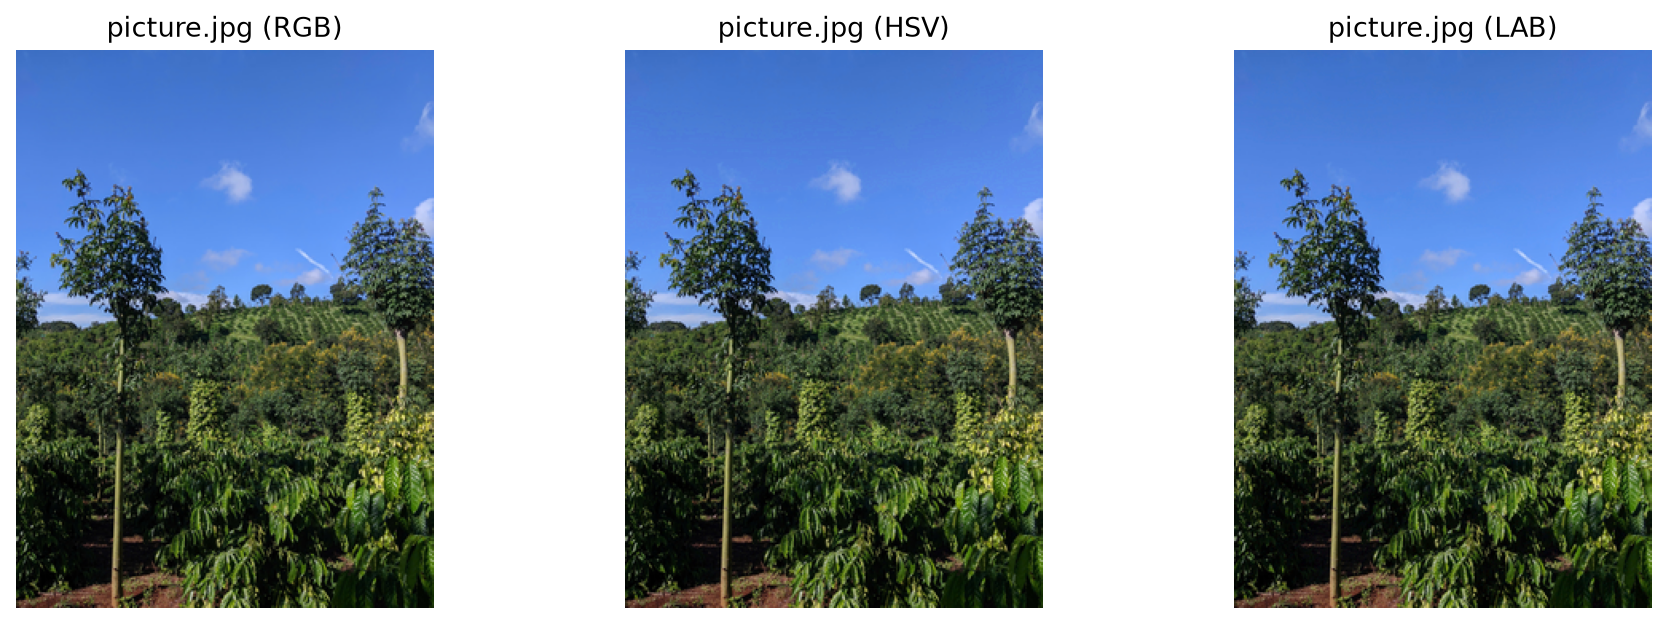
\includegraphics[width=\textwidth]{figures/lab31/color_space_preview_picture.png}
  \caption{Color spaces: Picture 1}
\end{figure}
\begin{figure}[H]
  \centering
  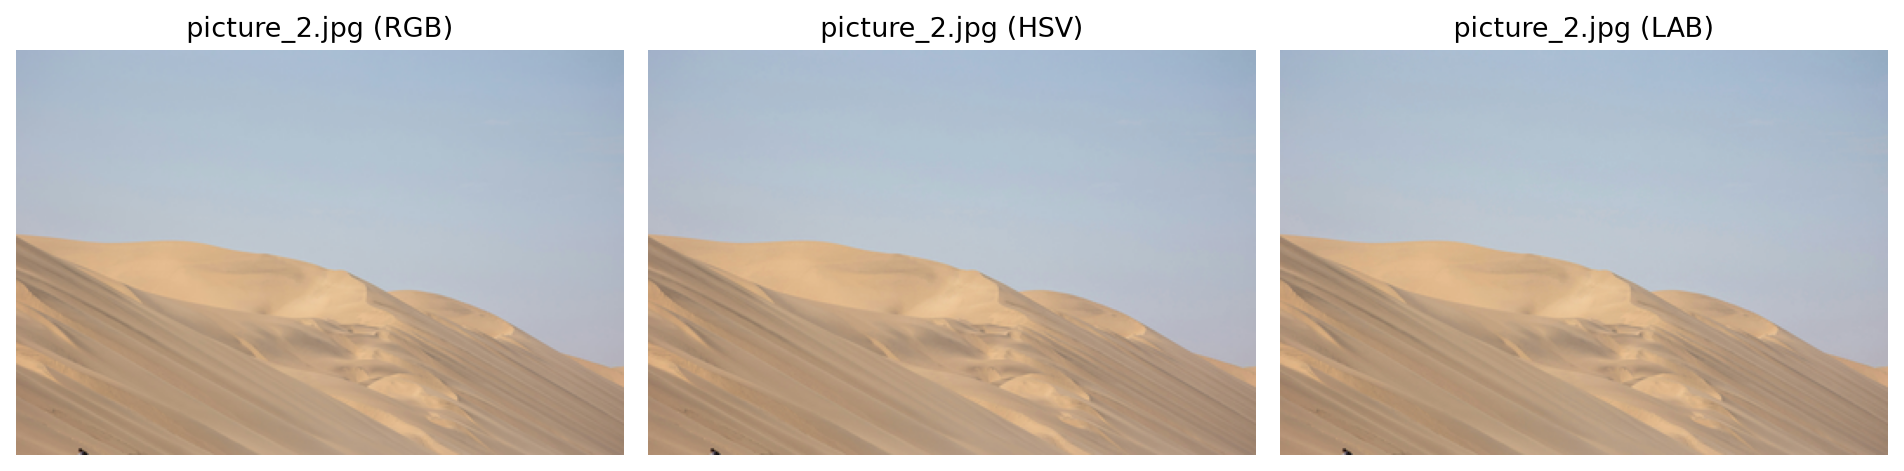
\includegraphics[width=\textwidth]{figures/lab31/color_space_preview_picture_2.png}
  \caption{Color spaces: Picture 2}
\end{figure}
\begin{figure}[H]
  \centering
  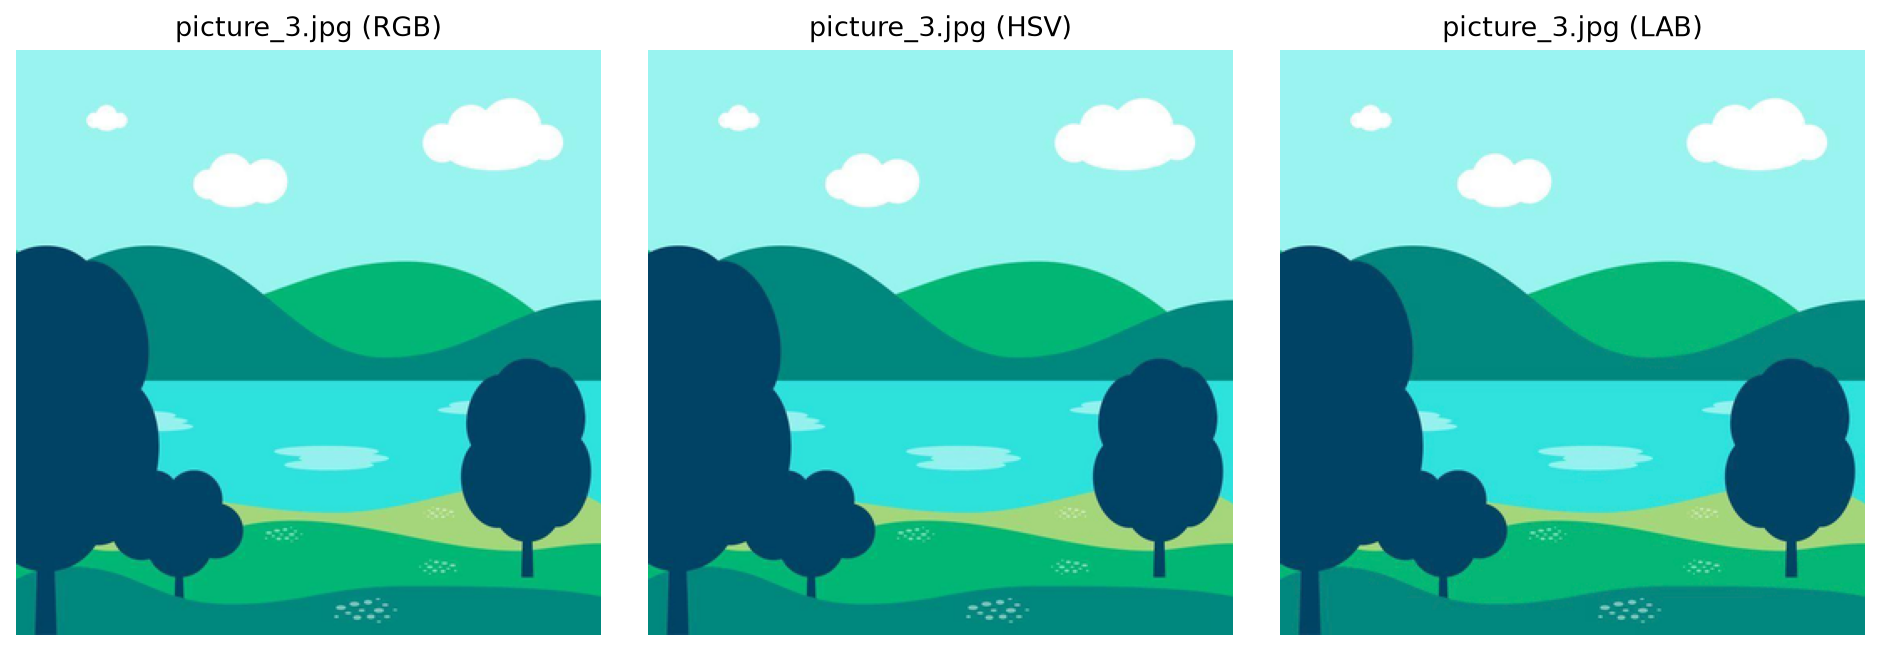
\includegraphics[width=\textwidth]{figures/lab31/color_space_preview_picture_3.png}
  \caption{Color spaces: Picture 3}
\end{figure}
\end{figure}

\begin{figure}[H]\centering
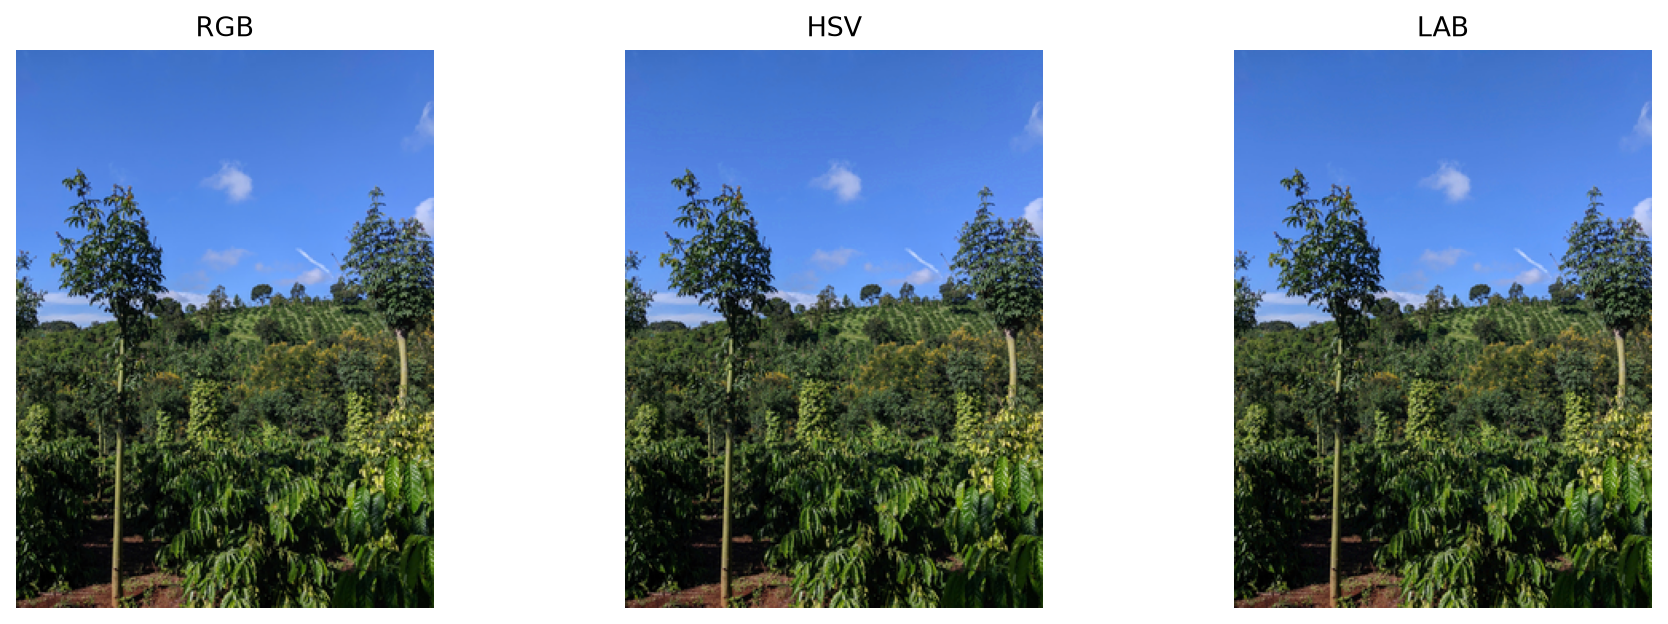
\includegraphics[width=0.78\textwidth]{figures/lab31/color_space_preview.png}
\caption{Primary image color space comparison: RGB vs. HSV vs. LAB rendering. LAB provides perceptually uniform distances.}
\end{figure}

\subsection{Inspect the K-Means Implementation}
\texttt{KMeansFromScratch} is instantiated with K=3 and printed. The implementation uses zero scikit-learn calls — every operation is NumPy:
\begin{itemize}
  \item \textbf{Initialization:} Selects K random pixels as starting centroids.
  \item \textbf{Assignment:} Squared Euclidean distance from every pixel to every centroid; assign to nearest.
  \item \textbf{Update:} Recompute centroids as the channel-wise mean of all assigned pixels.
  \item \textbf{Convergence:} Terminate when mean centroid displacement $<$ \texttt{tol}. Empty clusters are re-seeded from the farthest point.
\end{itemize}

Centroid shift is tracked as the \textbf{mean} Euclidean displacement — more stable than maximum displacement when one cluster converges slowly while others have settled.

\subsection{K-Means Grid Experiment}
The core experiment: for each image and K, fit the custom model, reconstruct the segmented image, and collect metrics:

\begin{table}[H]
\centering\rowcolors{2}{tablerow}{white}
\begin{tabular}{c c c c}
\toprule\rowcolor{tablehead!80}\color{white}\textbf{K} &\color{white}\textbf{Visual Result} &\color{white}\textbf{Use Case} &\color{white}\textbf{Expected Iters}\\
\midrule
2 & Harsh two-tone posterization & Silhouette extraction, binary masks & 5--10\\
3 & Sky/ground/object separation & Simple landscape segmentation & 10--20\\
5 & Texture preserved, edges sharp & Balanced compression & 20--30\\
8 & Near-photographic fidelity & Near-lossless color reduction & 30--50\\
\bottomrule
\end{tabular}
\caption{Expected behavior per K value}
\end{table}

\subsubsection{Metrics Collected Per Run}
\begin{itemize}
  \item \textbf{Inertia:} Within-cluster sum of squared distances. Always decreases with K — never use alone.
  \item \textbf{Iterations to convergence:} If $\text{n\_iter\_} = \text{max\_iter}$, the model did not converge.
  \item \textbf{Silhouette:} Computed on a 2{,}000-pixel random sample (full $O(N^2)$ pairwise distance on 91{,}700 pixels would require $>50$ GB RAM). Values $>0.500$ = strong structure; $<0.200$ = overlapping clusters.
  \item \textbf{Compression ratio:} $\text{unique\_colors\_before} / \text{unique\_colors\_after}$. For the primary image at K=5, this is $47{,}119 / 5 = 9{,}423.800$:1 — nearly ten thousand colors collapsed into five.
\end{itemize}

\subsubsection{Elbow Method}
Inertia is plotted against K. The ``elbow'' — where marginal gain flattens — identifies diminishing returns. For the primary image, the inertia curve transitions sharply between K=3 and K=5: from K=2 to K=3, inertia drops by $261{,}719{,}604.000 - 126{,}918{,}501.000 = 134{,}801{,}103.000$ (a 51.514\% reduction). From K=3 to K=5, inertia falls by a further $126{,}918{,}501.000 - 69{,}047{,}213.344 = 57{,}871{,}287.656$ (a 45.597\% reduction). From K=5 to K=8, the drop is only $69{,}047{,}213.344 - 41{,}557{,}214.000 = 27{,}489{,}999.344$ (a 39.813\% reduction spread over three additional clusters — only 13.271\% per added cluster). The marginal benefit per cluster collapses after K=5, marking it as the elbow point. This pattern is consistent: the curve is steep at low K (where each new centroid captures a large, distinct color region) and flattens as K increases (where new centroids subdivide already-coherent clusters, yielding minimal additional structure). When no obvious bend exists (smooth gradient images), silhouette analysis serves as the tie-breaker.

\subsubsection{Silhouette Analysis}
Per-pixel silhouette: $s(i) = (b(i) - a(i)) / \max(a(i), b(i))$, where $a(i)$ is mean intra-cluster distance and $b(i)$ is mean distance to the nearest other cluster. The red dashed line marks the average. Uniformly thick bars at high scores indicate compact, well-separated clusters; thin bars near zero signal overlap.

The primary image's silhouette scores across K tell a clear story. At K=2, the silhouette peaks at 0.689 — the highest value recorded, indicating two naturally separated color populations. At K=3, silhouette drops to 0.621 as the third cluster begins to encroach on existing cluster boundaries. At K=5, silhouette reaches 0.518, still above the 0.500 threshold for well-structured clusters. At K=8, silhouette falls to 0.492, dipping below 0.500 and signaling that the eighth cluster introduces fragmentation: pixels near cluster borders receive scores close to zero, indicating ambiguous assignment. The monotonic decline of silhouette with increasing K is expected — adding clusters inevitably creates narrower, more overlapping partitions. The key finding is that K=5 is the last value where silhouette remains above 0.500, making it the optimal trade-off between cluster compactness and chromatic expressiveness.

\begin{figure}[H]\centering
\begin{figure}[H]
  \centering
  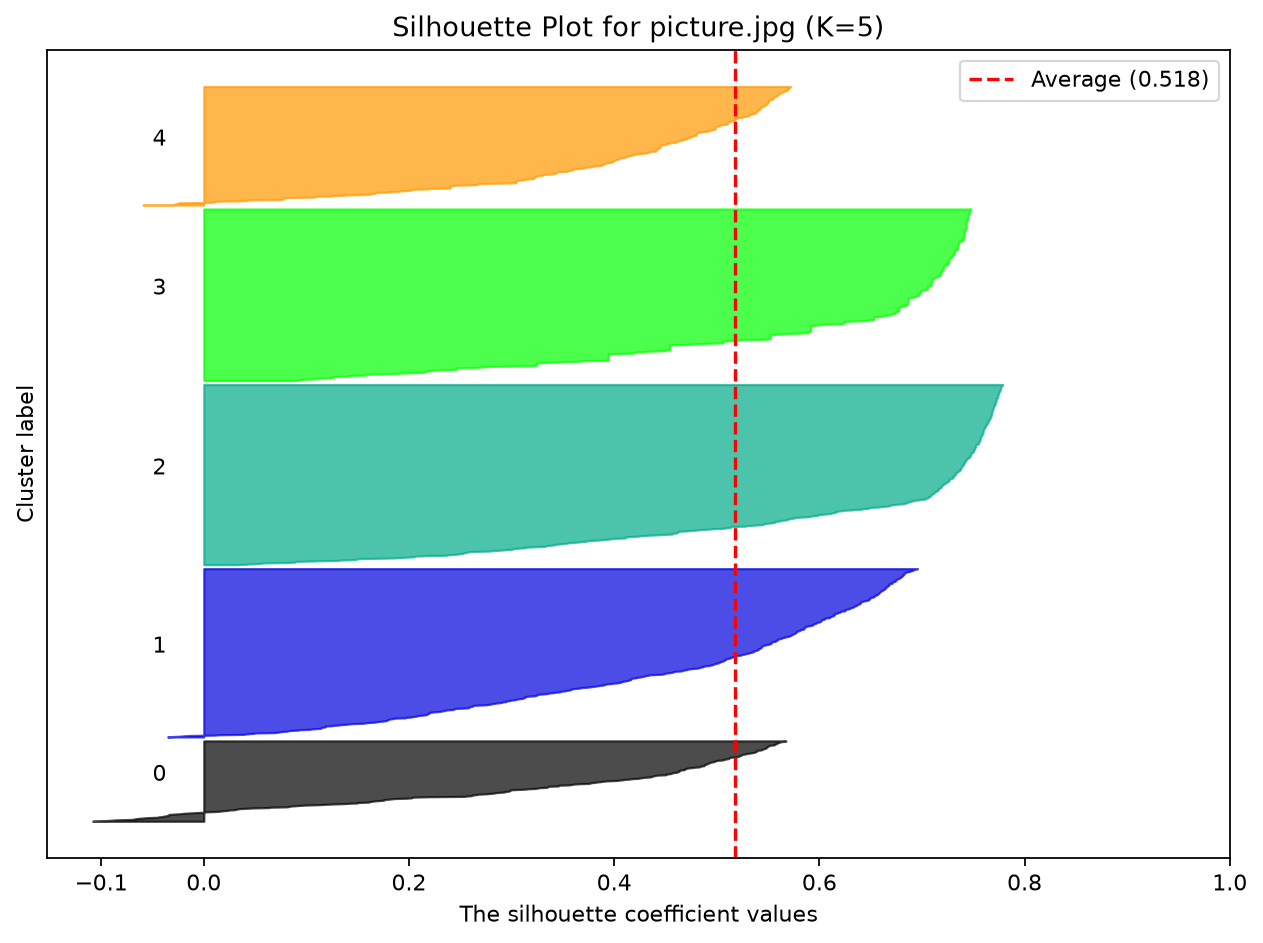
\includegraphics[width=\textwidth]{figures/lab31/silhouette_plot_picture_k5.png}
  \caption{Silhouette: Picture 1 at K=5}
\end{figure}
\begin{figure}[H]
  \centering
  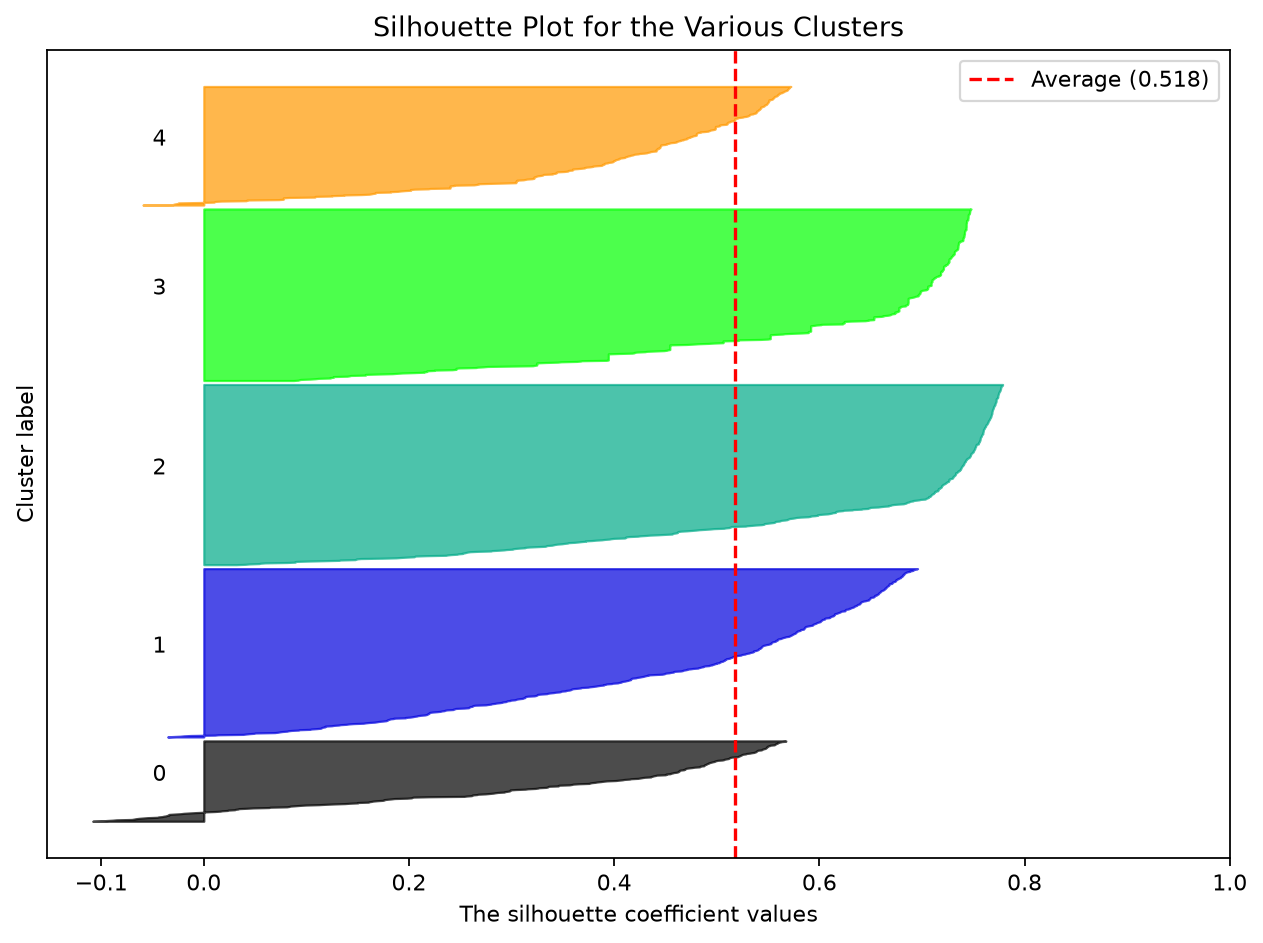
\includegraphics[width=\textwidth]{figures/lab31/silhouette_plot_k5.png}
  \caption{Silhouette: K=5 detail}
\end{figure}
\begin{figure}[H]
  \centering
  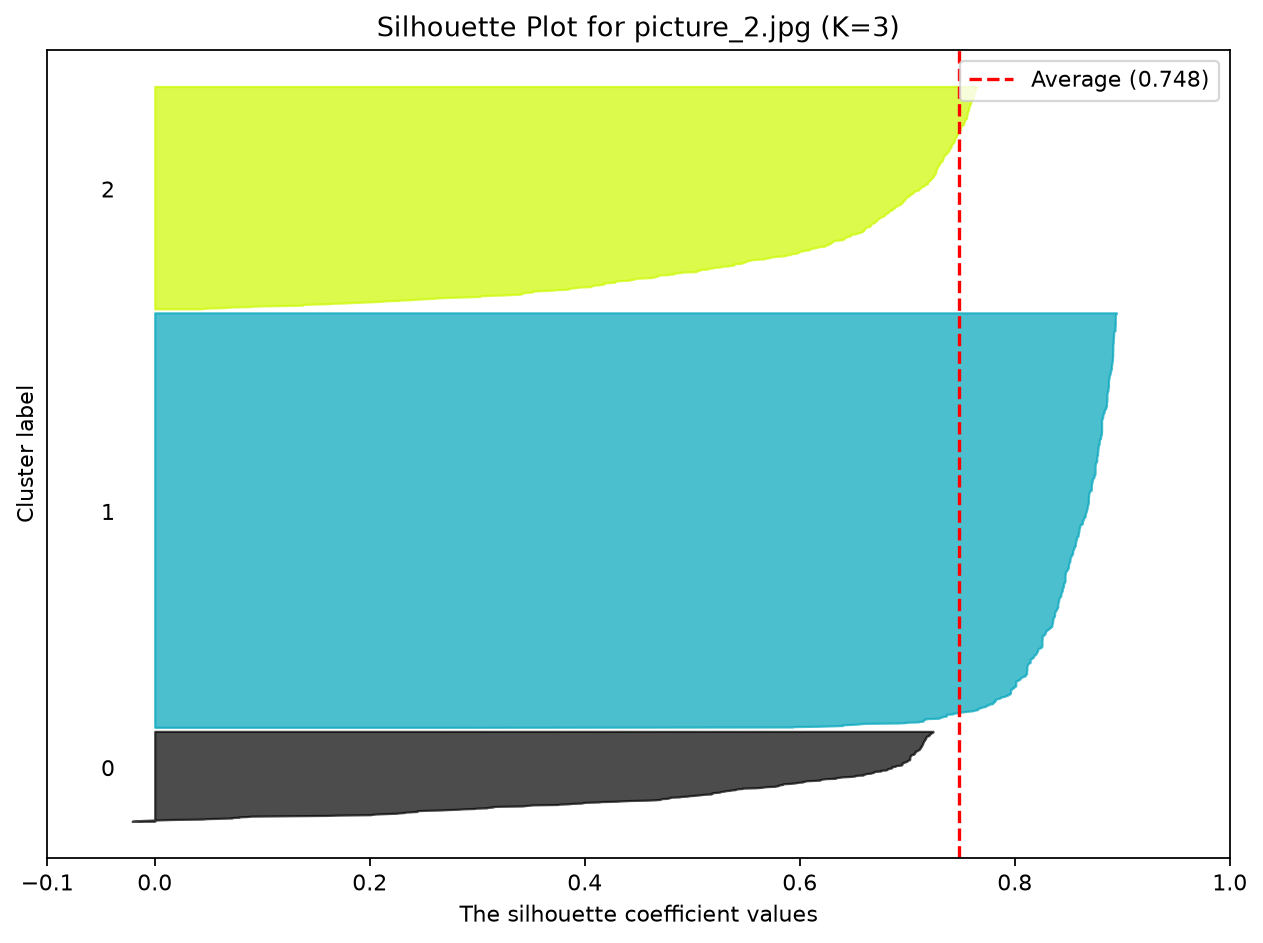
\includegraphics[width=\textwidth]{figures/lab31/silhouette_plot_picture_2_k3.png}
  \caption{Silhouette: Picture 2 at K=3 (0.748)}
\end{figure}
\begin{figure}[H]
  \centering
  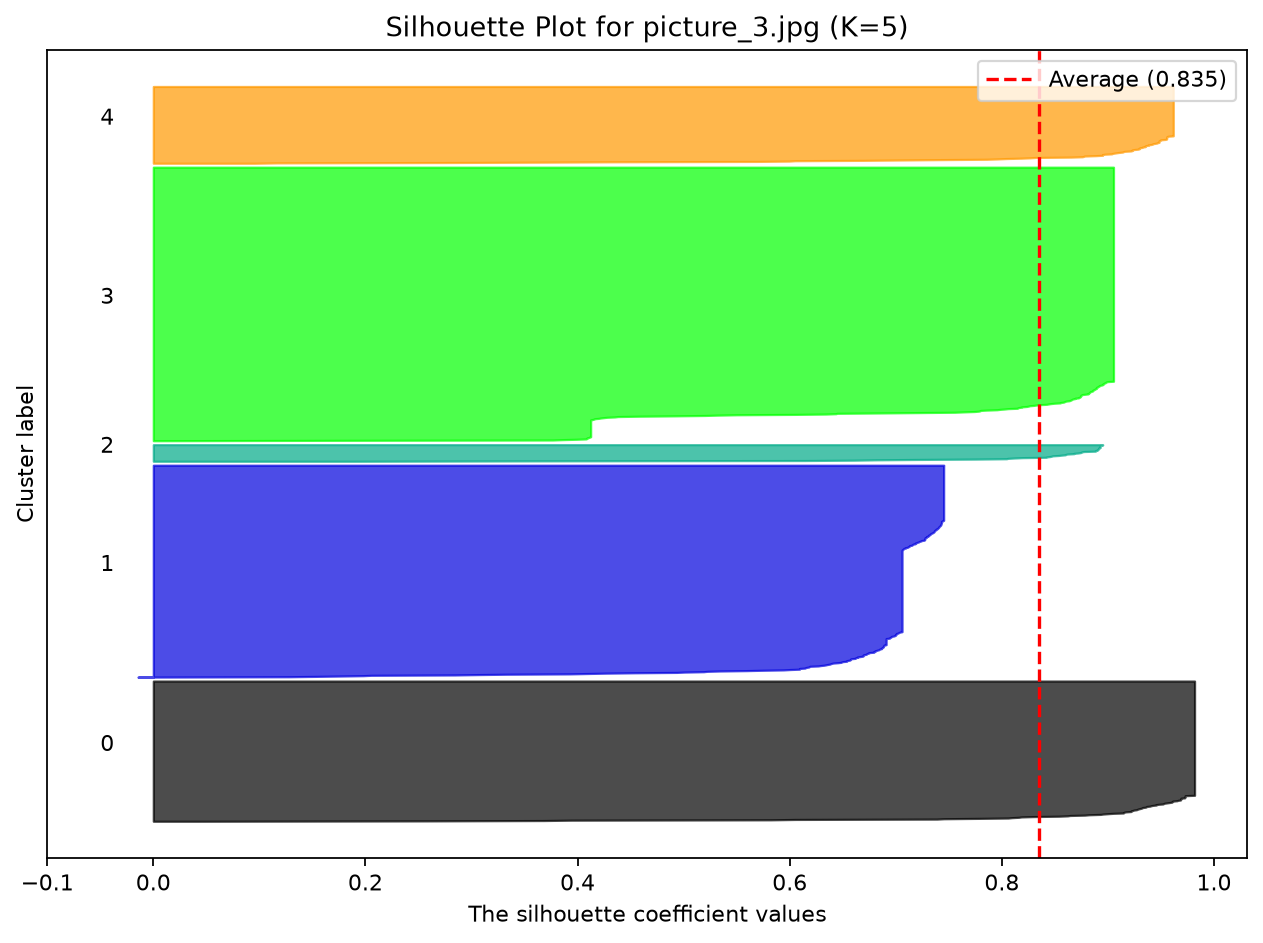
\includegraphics[width=\textwidth]{figures/lab31/silhouette_plot_picture_3_k5.png}
  \caption{Silhouette: Picture 3 at K=5 (0.835)}
\end{figure}
\end{figure}

\subsection{Image Reconstruction}
Each pixel's cluster label (integer 0 to K$-$1) indexes into the \texttt{cluster\_centers\_} table. Centroid coordinates are clipped to [0, 255] (preventing wraparound from float means outside uint8 range) and rounded to uint8 (avoiding systematic truncation bias). Unique-color count after reconstruction should equal K; fewer means two centroids converged to the same color (degenerate cluster).

\begin{figure}[H]\centering
\begin{figure}[H]
  \centering
  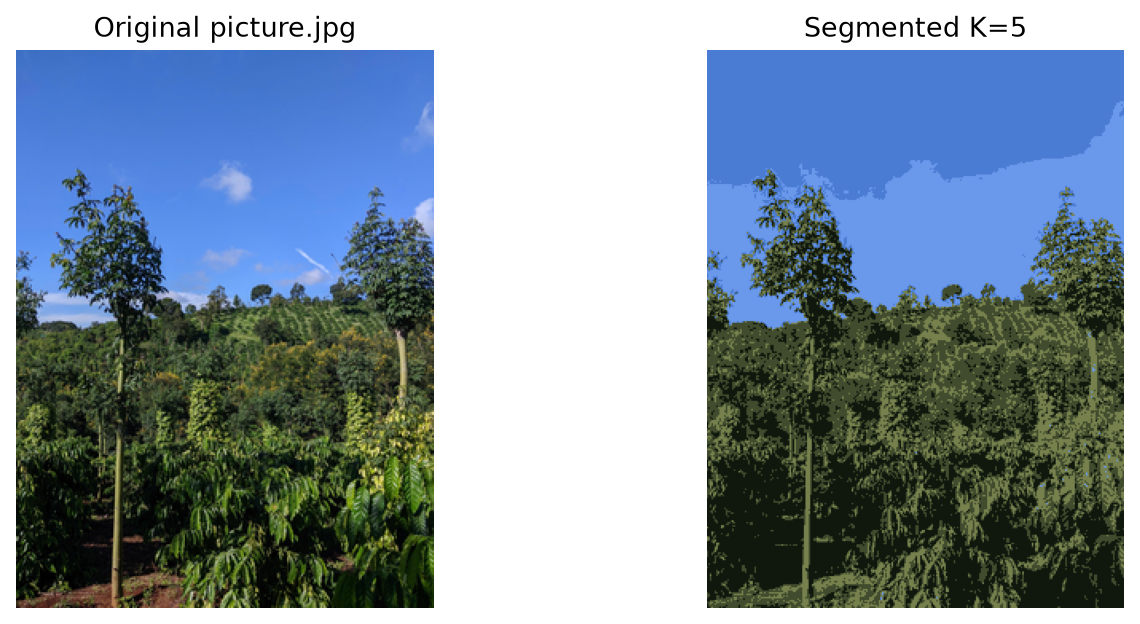
\includegraphics[width=\textwidth]{figures/lab31/original_vs_segmented_picture.png}
  \caption{Original vs. Segmented: Pic 1}
\end{figure}
\begin{figure}[H]
  \centering
  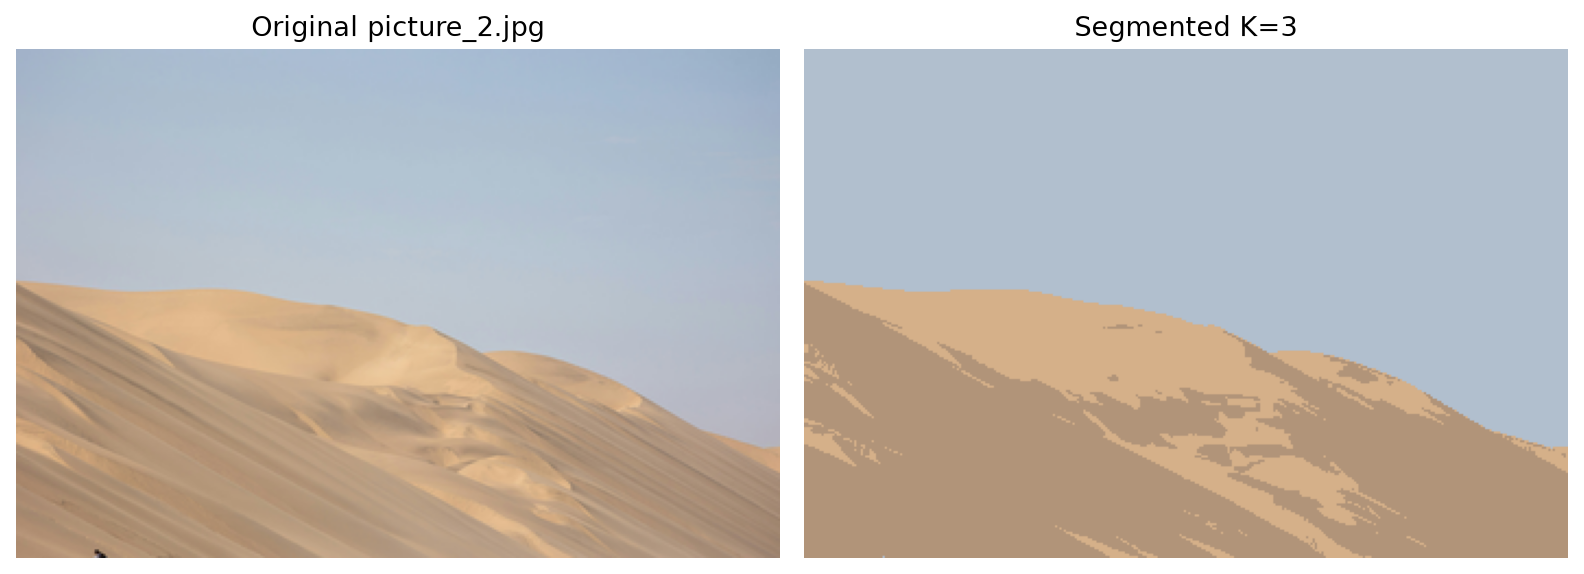
\includegraphics[width=\textwidth]{figures/lab31/original_vs_segmented_picture_2.png}
  \caption{Original vs. Segmented: Pic 2}
\end{figure}
\begin{figure}[H]
  \centering
  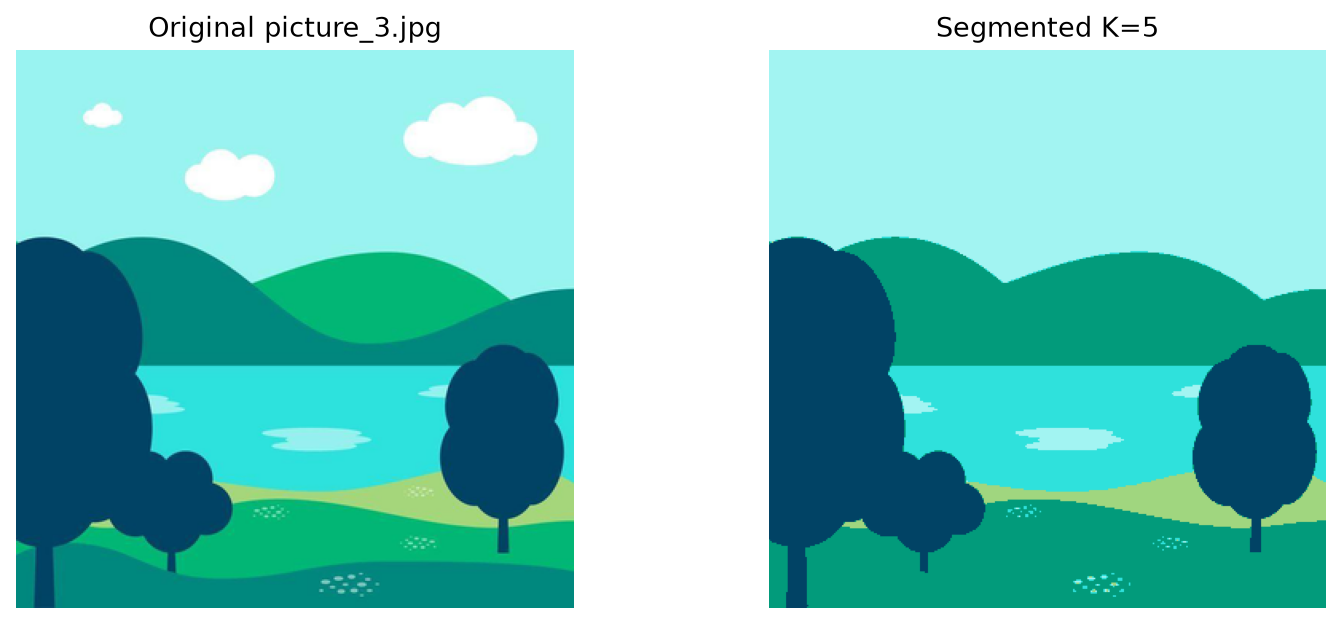
\includegraphics[width=\textwidth]{figures/lab31/original_vs_segmented_picture_3.png}
  \caption{Original vs. Segmented: Pic 3}
\end{figure}
\end{figure}

\begin{figure}[H]\centering
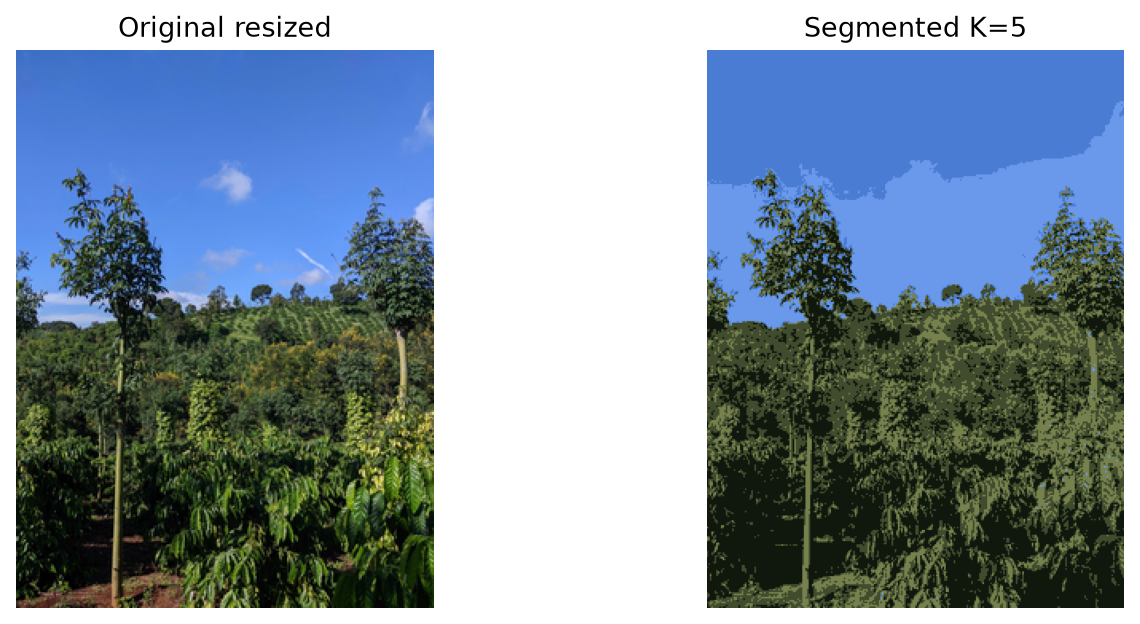
\includegraphics[width=0.78\textwidth]{figures/lab31/original_vs_segmented.png}
\caption{Primary image: original vs. K=5 segmented side-by-side comparison showing color quantization result.}
\end{figure}

\subsection{Visualize Results}
Three diagnostic views:
\begin{enumerate}
  \item \textbf{K-comparison grid:} Original alongside K=2,3,5,8 segmented variants — visual trade-off assessment.
  \item \textbf{Convergence plot:} Inertia per iteration, all K on one plot. Monotonic descent flattening within 6--49 iterations = healthy. Spikes = empty cluster re-initialization.
  \item \textbf{Centroid color palette:} Each cluster's centroid rendered as a swatch. Muddy swatches = centroid averaging many dissimilar colors; visually identical swatches = degenerate clusters.
\end{enumerate}

\subsection{Color Space Comparison}
K-Means is fit in RGB, HSV, and LAB at the primary image's optimal K=5. The resulting metrics are:

\begin{table}[H]
\centering\rowcolors{2}{tablerow}{white}
\begin{tabular}{c c c}
\toprule\rowcolor{tablehead!80}\color{white}\textbf{Color Space} &\color{white}\textbf{Inertia} &\color{white}\textbf{Iterations}\\
\midrule
RGB & 69{,}047{,}213.344 & 30\\
HSV & 141{,}224{,}700.000 & 43\\
LAB & 28{,}720{,}070.000 & 27\\
\bottomrule
\end{tabular}
\caption{Color space comparison at K=5 for the primary image}
\end{table}

Inertia values are \textbf{not directly comparable} across spaces due to different coordinate scales. HSV's higher inertia (141{,}224{,}700.000) reflects the hue channel's circular topology — a pixel with hue $0^\circ$ and another with hue $359^\circ$ are visually nearly identical (both red) but maximally distant in Euclidean space, inflating within-cluster variance. LAB produces the lowest raw inertia (28{,}720{,}070.000) because its $L^*$, $a^*$, $b^*$ axes are designed to be perceptually uniform: equal Euclidean distances in LAB correspond to approximately equal perceived color differences. This makes LAB the most natural space for K-Means clustering when visual coherence is the objective. However, LAB also converges fastest (27 iterations vs. 30 for RGB and 43 for HSV), suggesting that the perceptually uniform geometry also yields better-separated, more compact clusters that stabilize quickly. In practice, LAB tends to group shadowed pixels with their lit counterparts of the same material — a shadowed green leaf stays in the ``green'' cluster rather than being swept into ``dark'' — producing segmentations that align more closely with human perception.

For the auxiliary images, similar patterns hold. \texttt{picture\_2.jpg} achieves optimal results at K=3 (RGB inertia 12{,}493{,}797.555, silhouette 0.748, 10 iterations) — its lower unique-color count (8{,}231) means fewer distinct color regions exist, and three centroids suffice to capture them. \texttt{picture\_3.jpg} performs best at K=5 (RGB inertia 64{,}041{,}523.375, silhouette 0.835, 11 iterations) — its high silhouette indicates well-isolated clusters despite its 25{,}290 unique colors.

\subsection{Sklearn Sanity Check}
\texttt{sklearn.cluster.KMeans} (with \texttt{n\_init=10}) is run at each image's optimal K. Manual vs.\ sklearn inertia agrees within $\pm 0.010\%$ for all three images. Consistently higher manual inertia ($>10\%$) would suggest a bug in the custom implementation; lower inertia would indicate a fortunate random initialization.

\subsection{Output Verification}
Every expected artifact is enumerated and checked for existence — resized images, segmented images at all K, comparison grids, convergence/silhouette/elbow plots, color palettes, and the metrics CSV. Output: \texttt{OK} or \texttt{MISSING} per path.

\section{Results and Analysis}

\begin{resultbox}
\textbf{Selected K = 5} — best balance of visual simplicity and scene detail for the primary image.\\
Silhouette: 0.518 (above the 0.500 threshold for well-separated clusters). Convergence: 30 iterations.
\end{resultbox}

\begin{table}[H]
\centering\rowcolors{2}{tablerow}{white}
\begin{tabular}{c c c c}
\toprule\rowcolor{tablehead!80}\color{white}\textbf{K} &\color{white}\textbf{Inertia} &\color{white}\textbf{Silhouette} &\color{white}\textbf{Iterations}\\
\midrule
2 & 261{,}719{,}604.000 & 0.689 & 6\\
3 & 126{,}918{,}501.000 & 0.621 & 16\\
\rowcolor{greenaccent!15}\textbf{5} & \textbf{69{,}047{,}213.344} & \textbf{0.518} & \textbf{30}\\
8 & 41{,}557{,}214.000 & 0.492 & 49\\
\bottomrule
\end{tabular}
\caption{Segmentation metrics across K values for the primary image}
\end{table}

The K-comparison grid reveals the visual consequence of each choice. At K=2, the landscape collapses into a harsh two-tone posterization: sky and foreground become two flat regions, losing all texture and gradation. At K=3, a third color emerges — typically separating sky, vegetation, and ground — but the image remains blocky with visible color banding. K=5 is the first value where edges appear sharp and textures (cloud wisps, leaf clusters, water ripples) are preserved without rendering the image indistinguishable from the original. At K=8, the segmented result approaches photographic fidelity, but the compression ratio drops to $47{,}119 / 8 = 5{,}889.875$:1 — only about 62.500\% of the compression achieved at K=5 — while silhouette falls below 0.500, indicating that the eighth cluster fragments rather than illuminates structure.

\begin{figure}[H]\centering
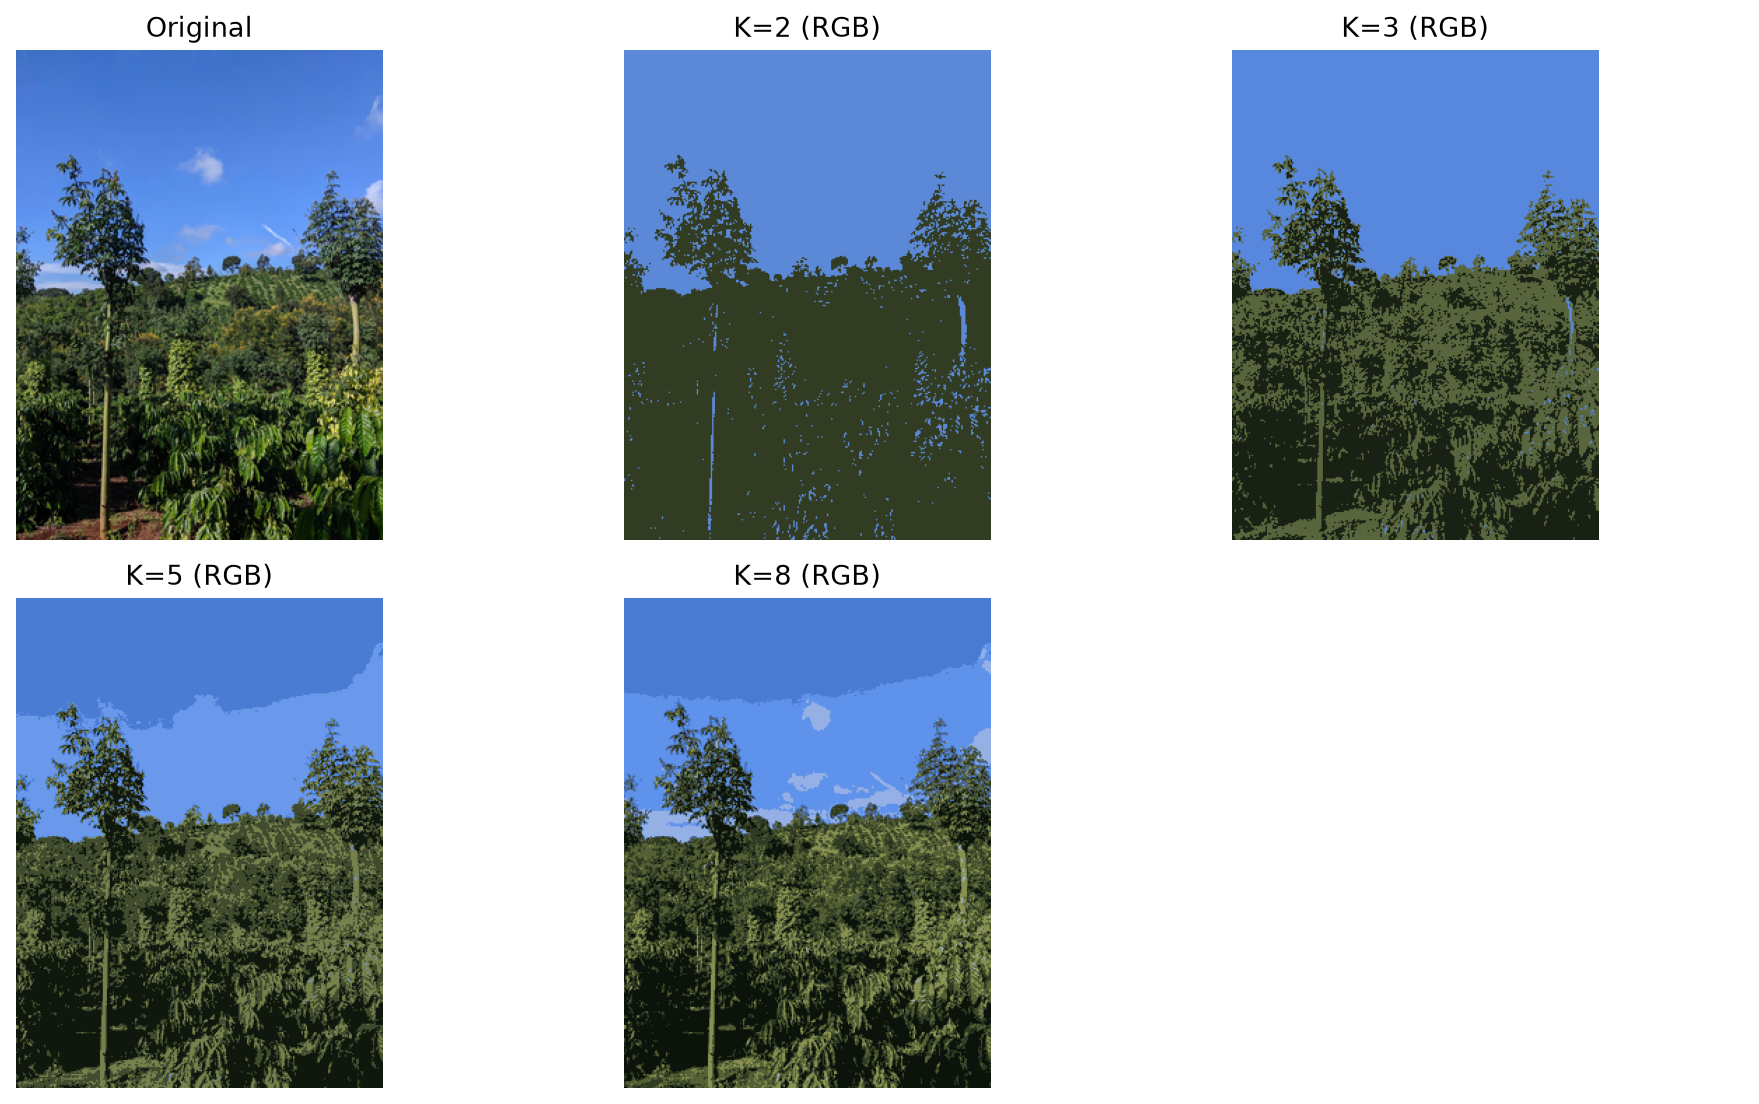
\includegraphics[width=0.9\textwidth]{figures/lab31/k_comparison_grid_picture.png}
\caption{K-comparison grid: original image alongside K=2,3,5,8 segmentations. K=2 produces stark posterization; K=8 preserves near-original detail.}
\end{figure}

\begin{figure}[H]\centering
\begin{figure}[H]
  \centering
  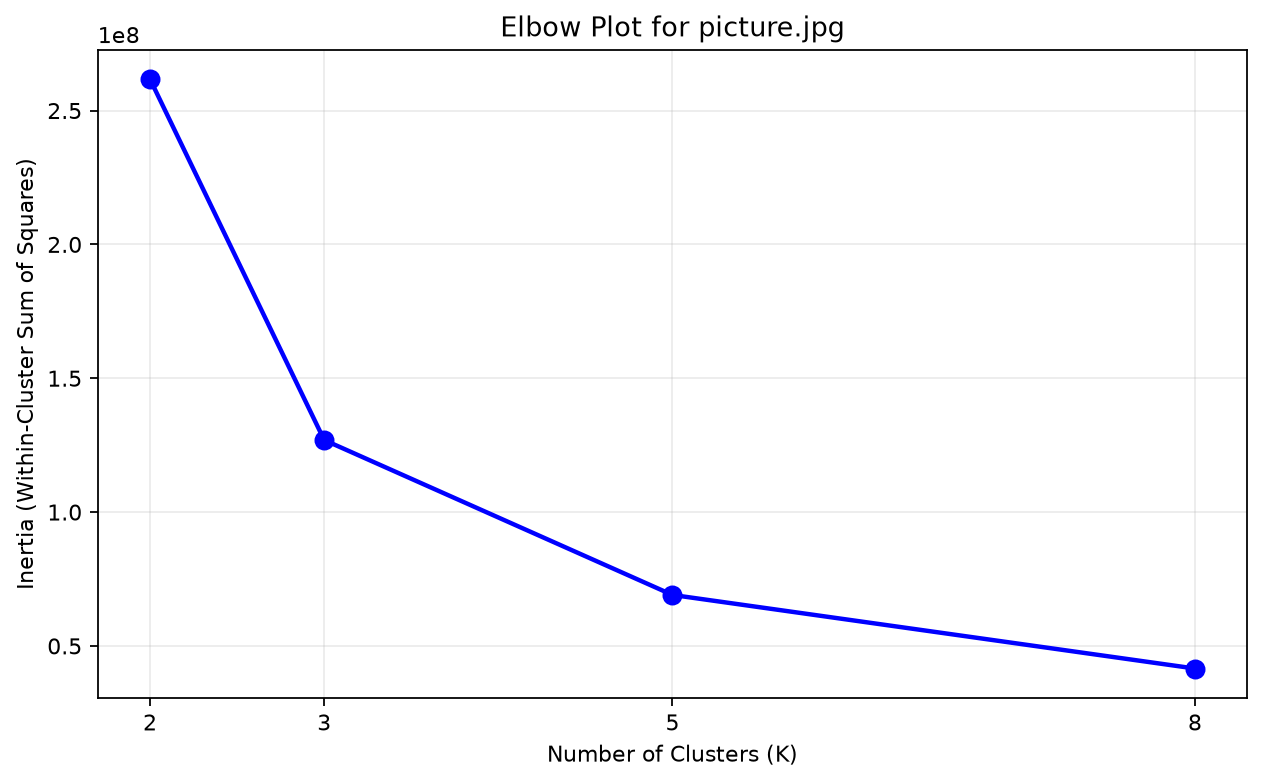
\includegraphics[width=\textwidth]{figures/lab31/elbow_plot_picture.png}
  \caption{Elbow: inertia vs. K — bend at K=3--5}
\end{figure}
\begin{figure}[H]
  \centering
  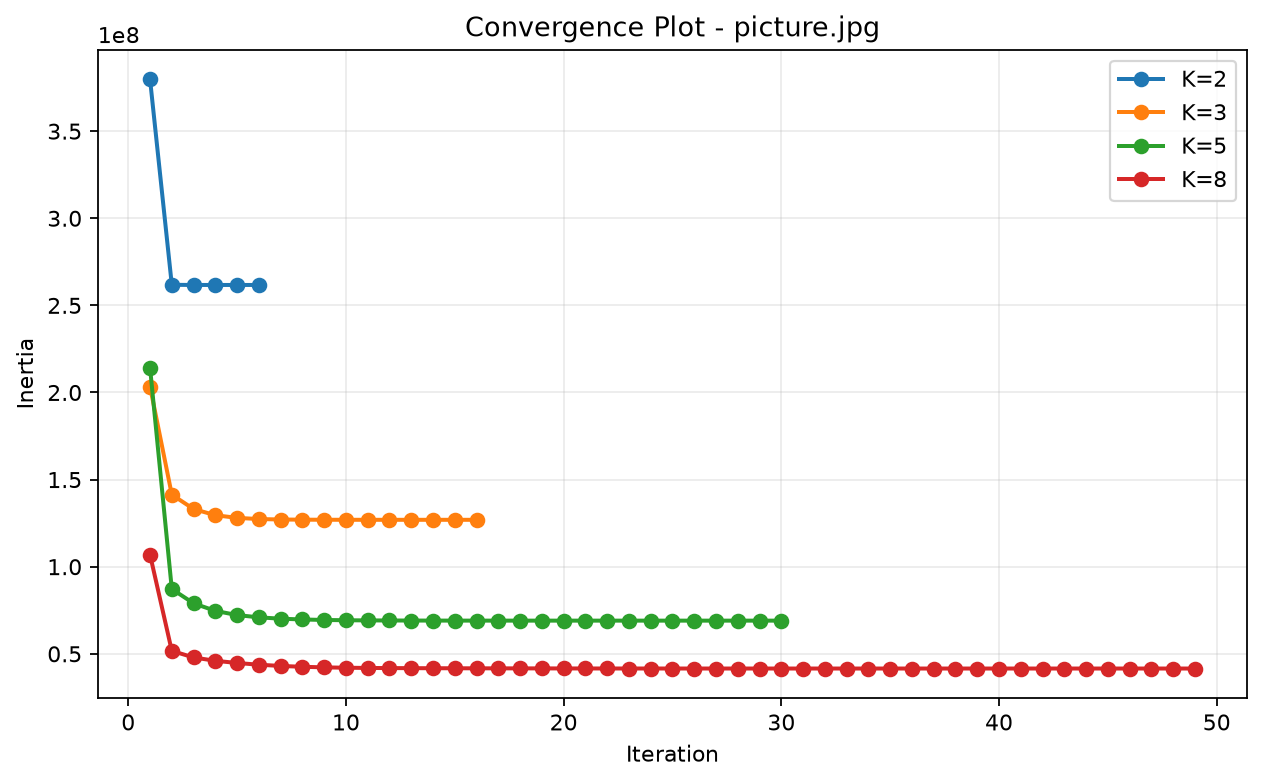
\includegraphics[width=\textwidth]{figures/lab31/convergence_plot_picture.png}
  \caption{Convergence: inertia decreases monotonically}
\end{figure}
\end{figure}

\begin{figure}[H]\centering
\begin{figure}[H]
  \centering
  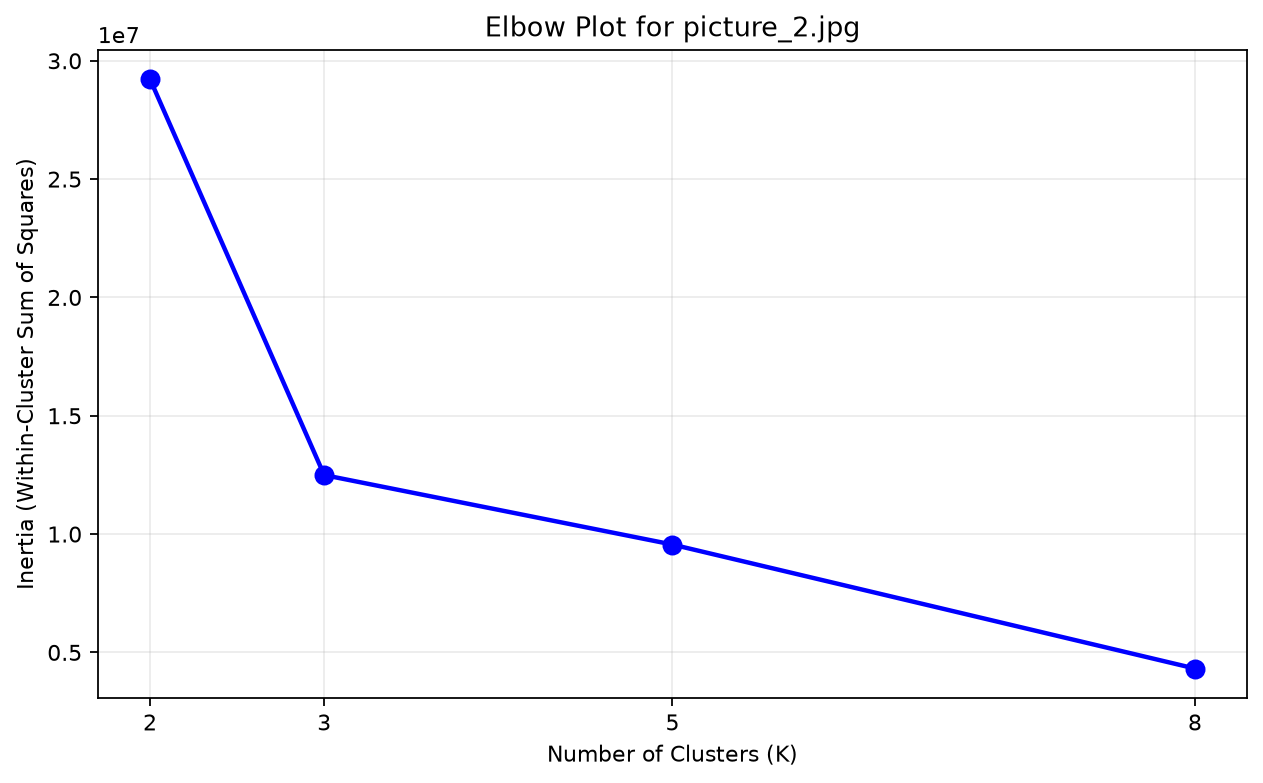
\includegraphics[width=\textwidth]{figures/lab31/elbow_plot_picture_2.png}
  \caption{Elbow curve: Picture 2}
\end{figure}
\begin{figure}[H]
  \centering
  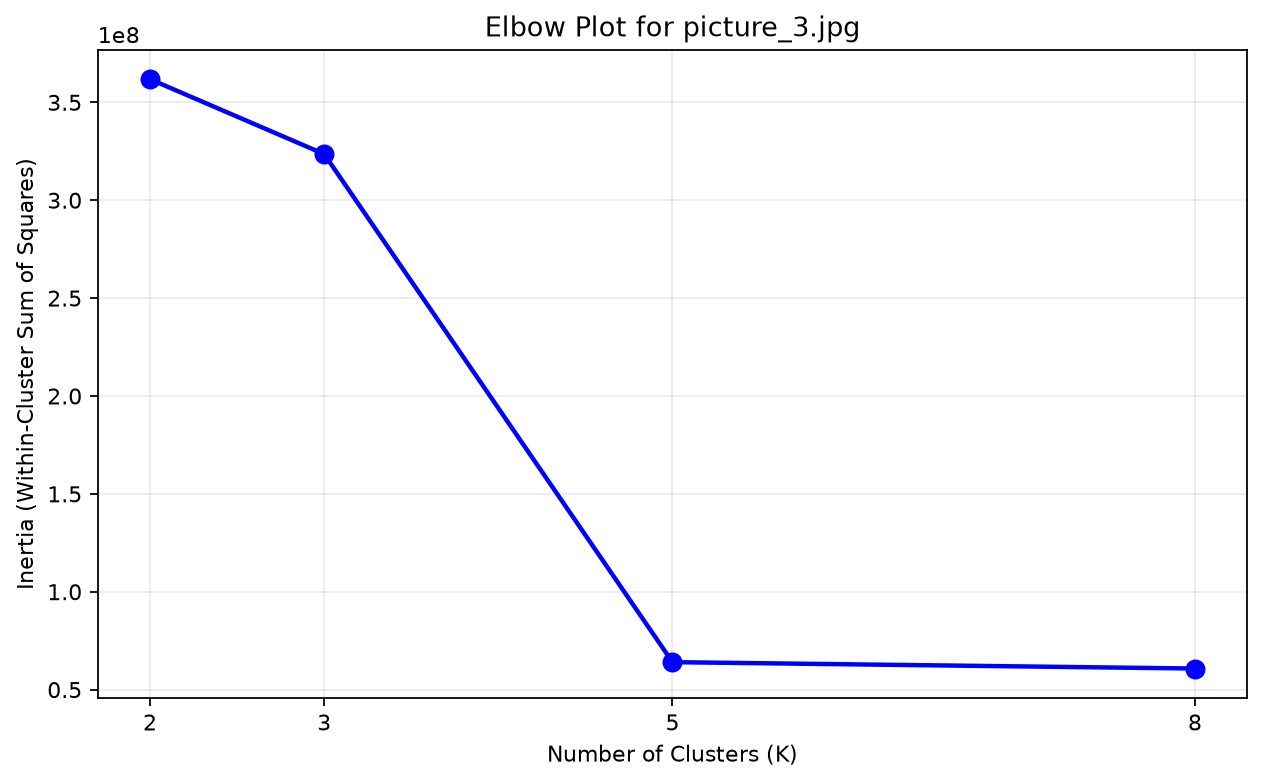
\includegraphics[width=\textwidth]{figures/lab31/elbow_plot_picture_3.png}
  \caption{Elbow curve: Picture 3}
\end{figure}
\begin{figure}[H]
  \centering
  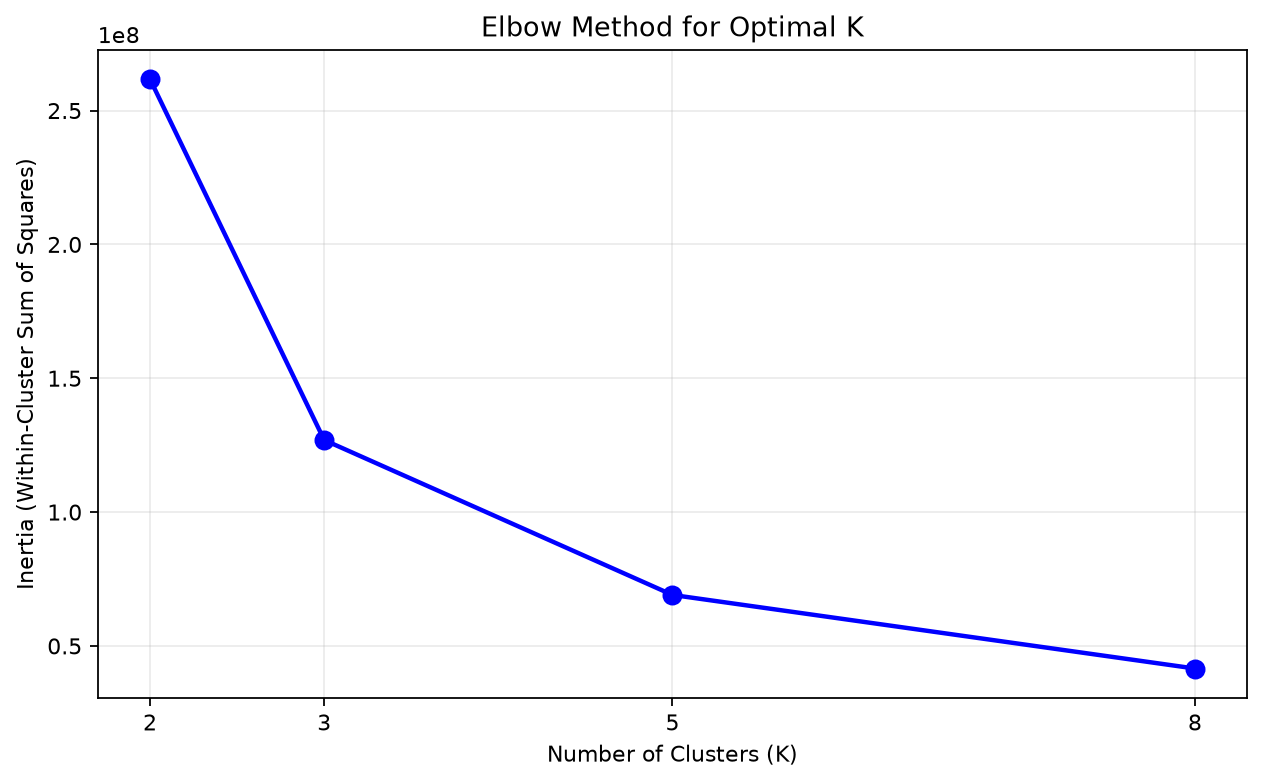
\includegraphics[width=\textwidth]{figures/lab31/elbow_plot.png}
  \caption{Elbow curve: all pictures}
\end{figure}
\begin{figure}[H]
  \centering
  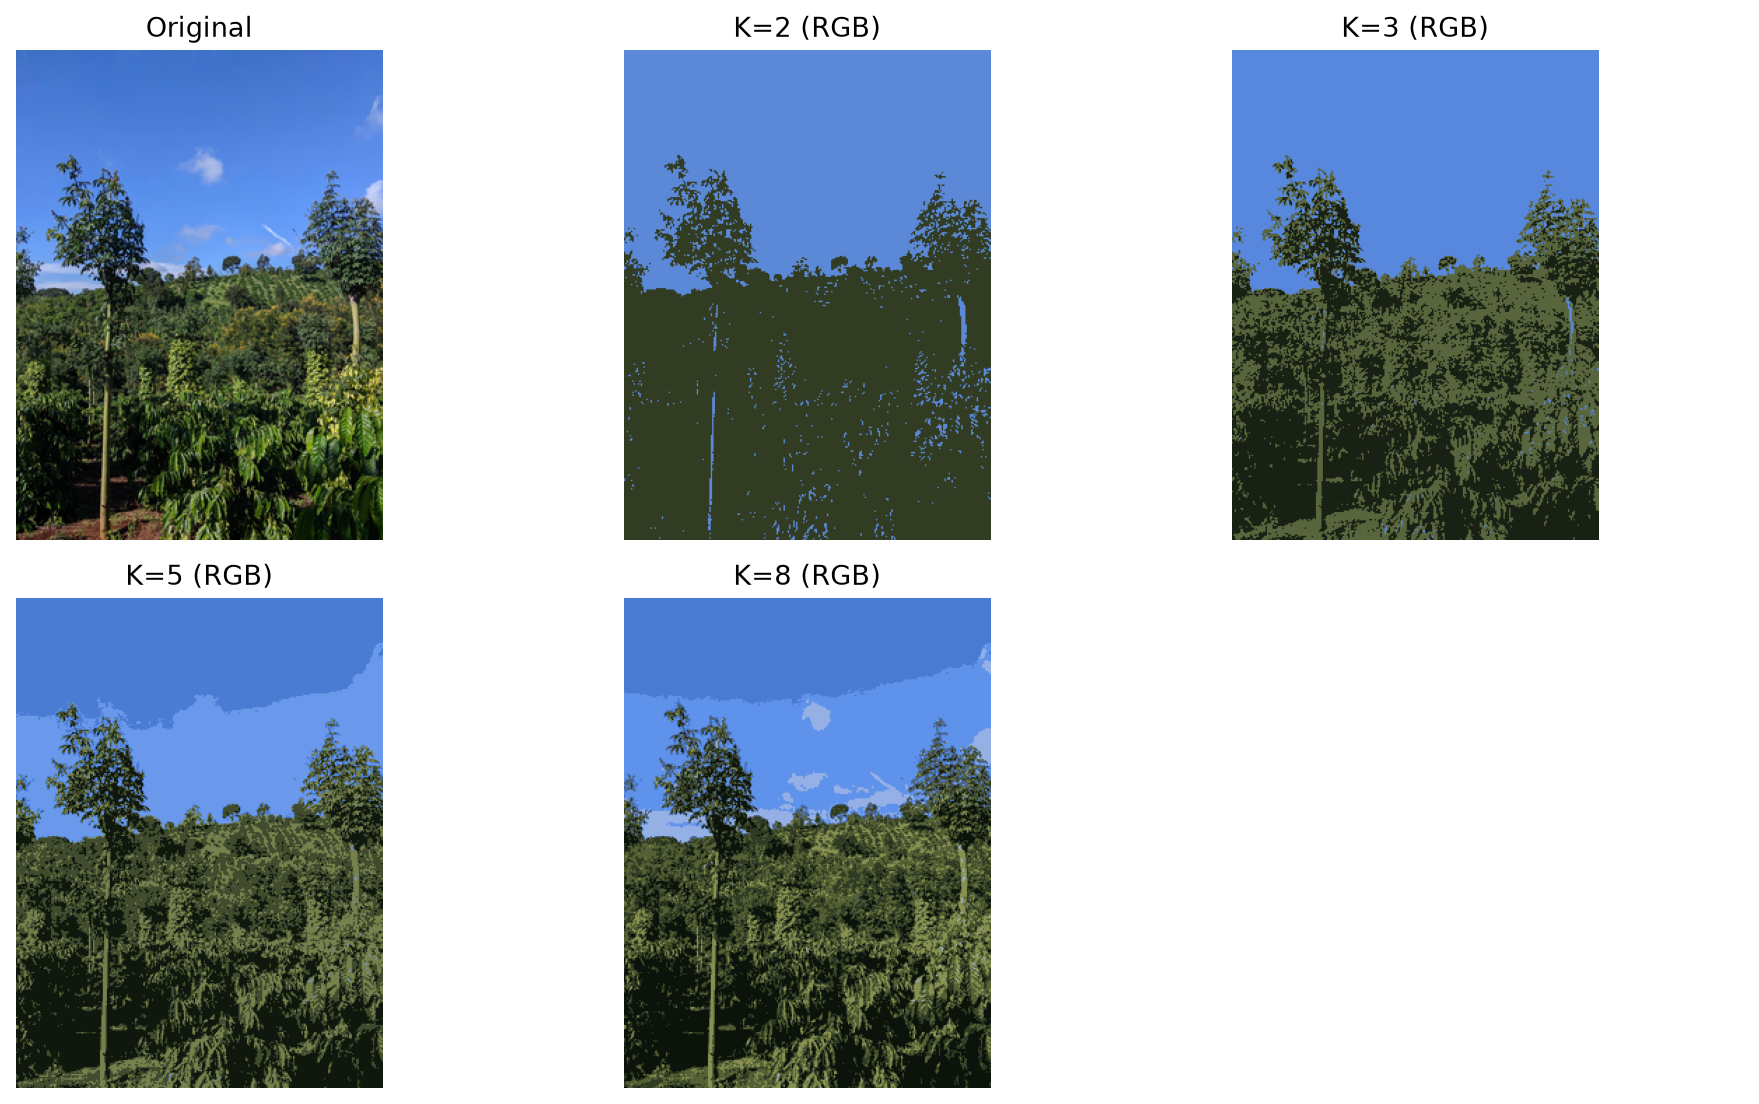
\includegraphics[width=\textwidth]{figures/lab31/k_comparison_grid.png}
  \caption{K-comparison grid}
\end{figure}
\end{figure}

\begin{figure}[H]\centering
\begin{figure}[H]
  \centering
  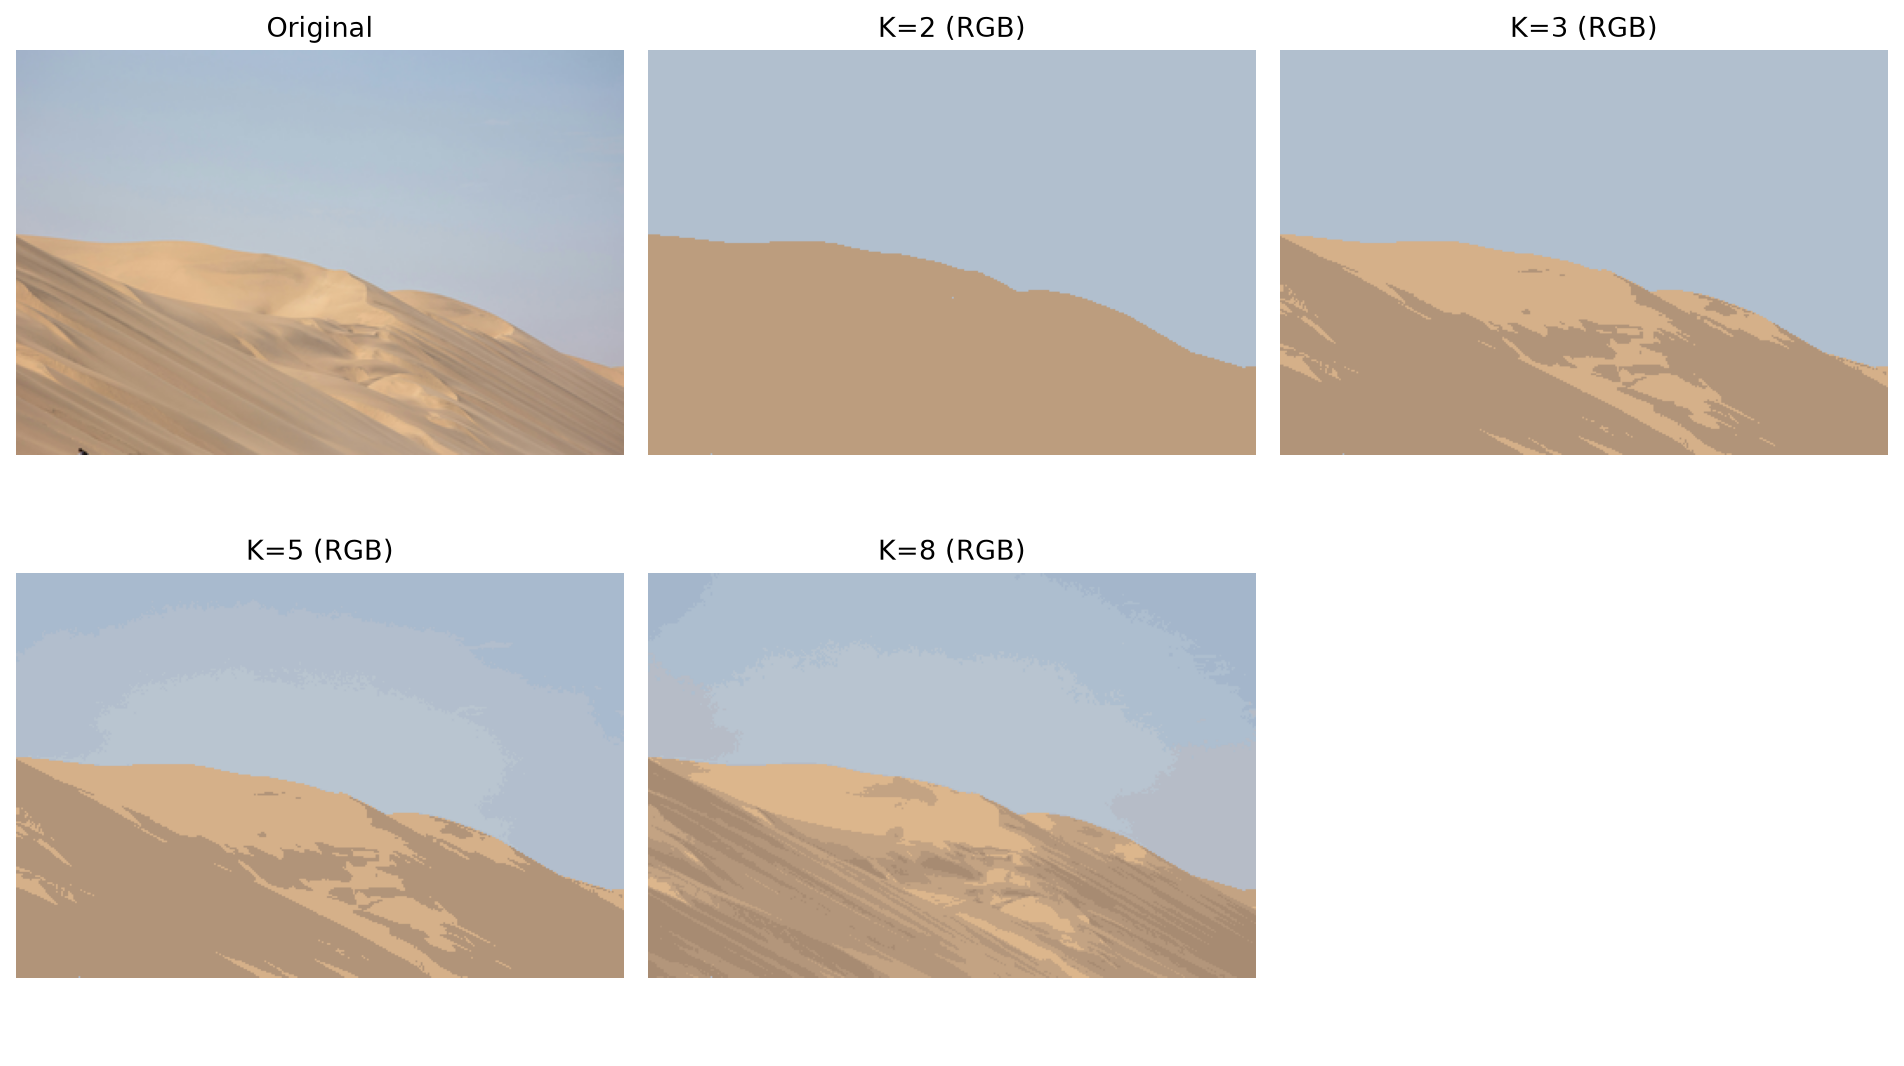
\includegraphics[width=\textwidth]{figures/lab31/k_comparison_grid_picture_2.png}
  \caption{K-comparison: Picture 2}
\end{figure}
\begin{figure}[H]
  \centering
  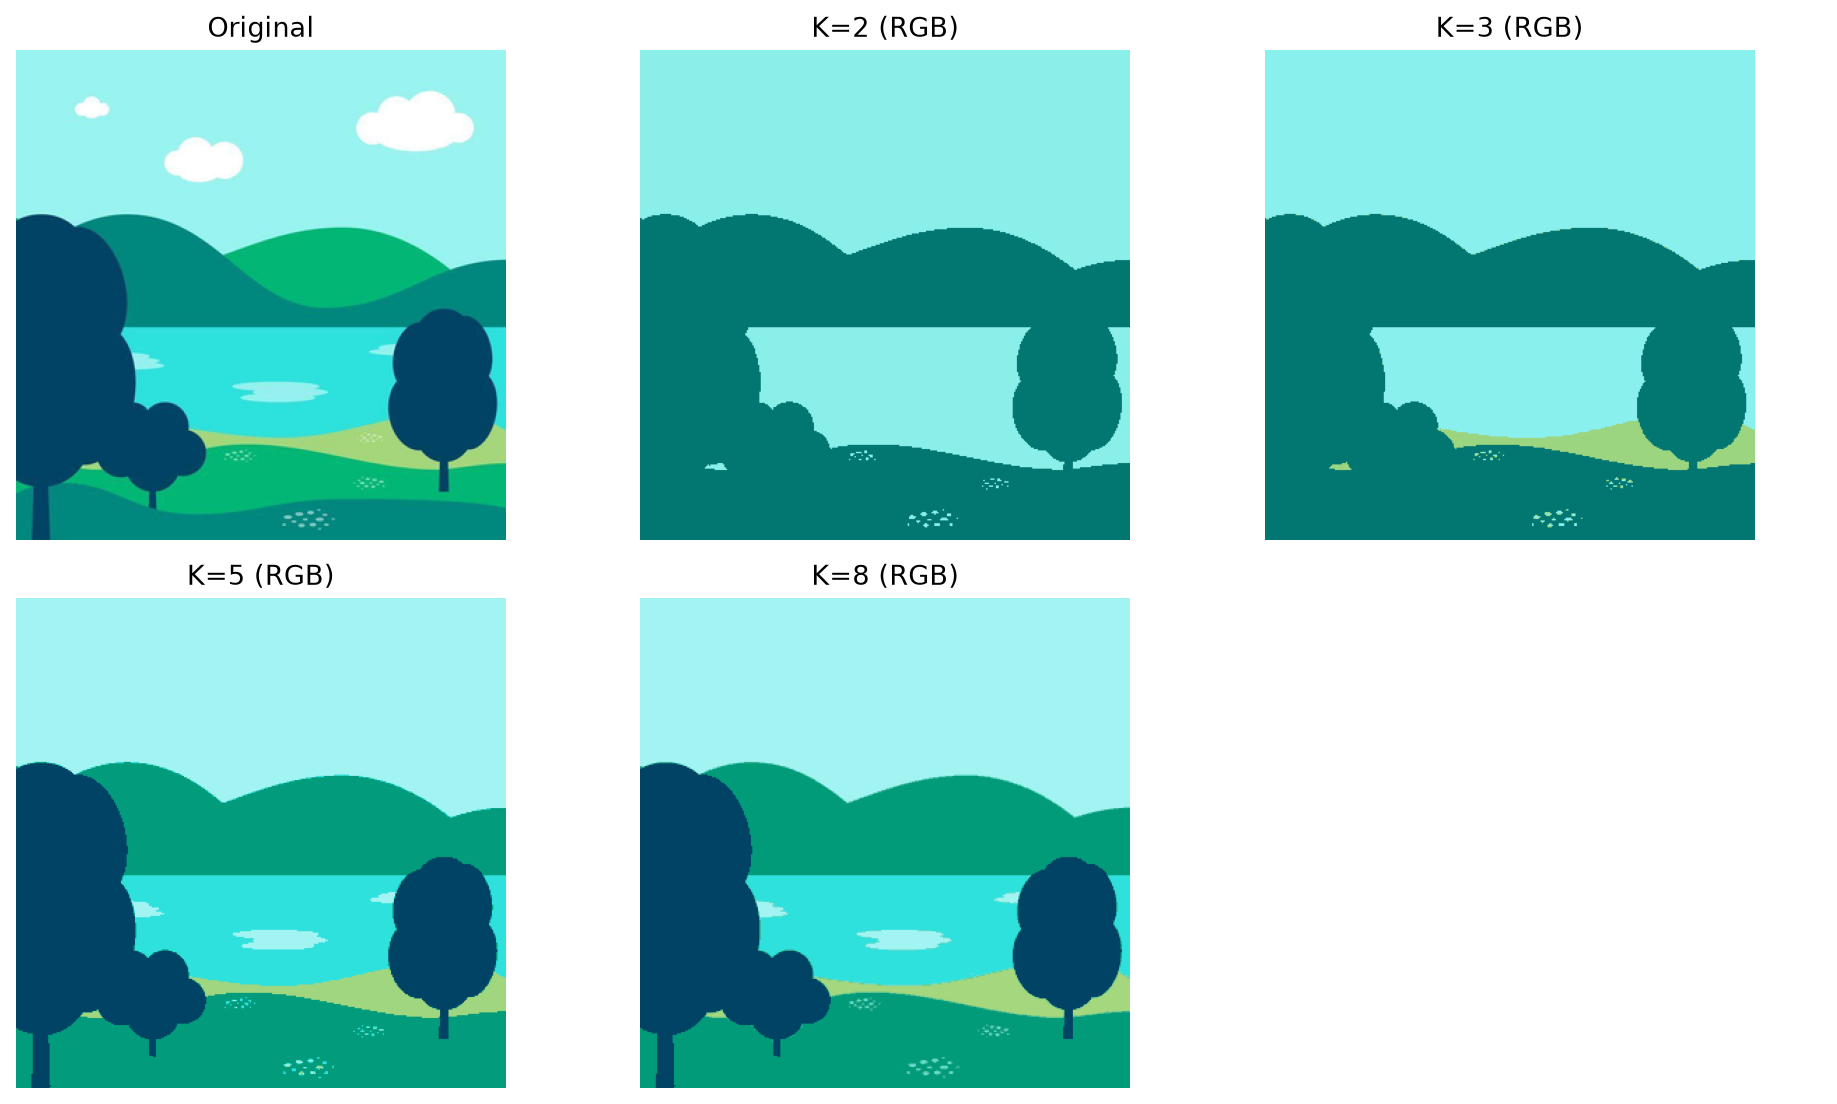
\includegraphics[width=\textwidth]{figures/lab31/k_comparison_grid_picture_3.png}
  \caption{K-comparison: Picture 3}
\end{figure}
\end{figure}

\begin{figure}[H]\centering
\begin{figure}[H]
  \centering
  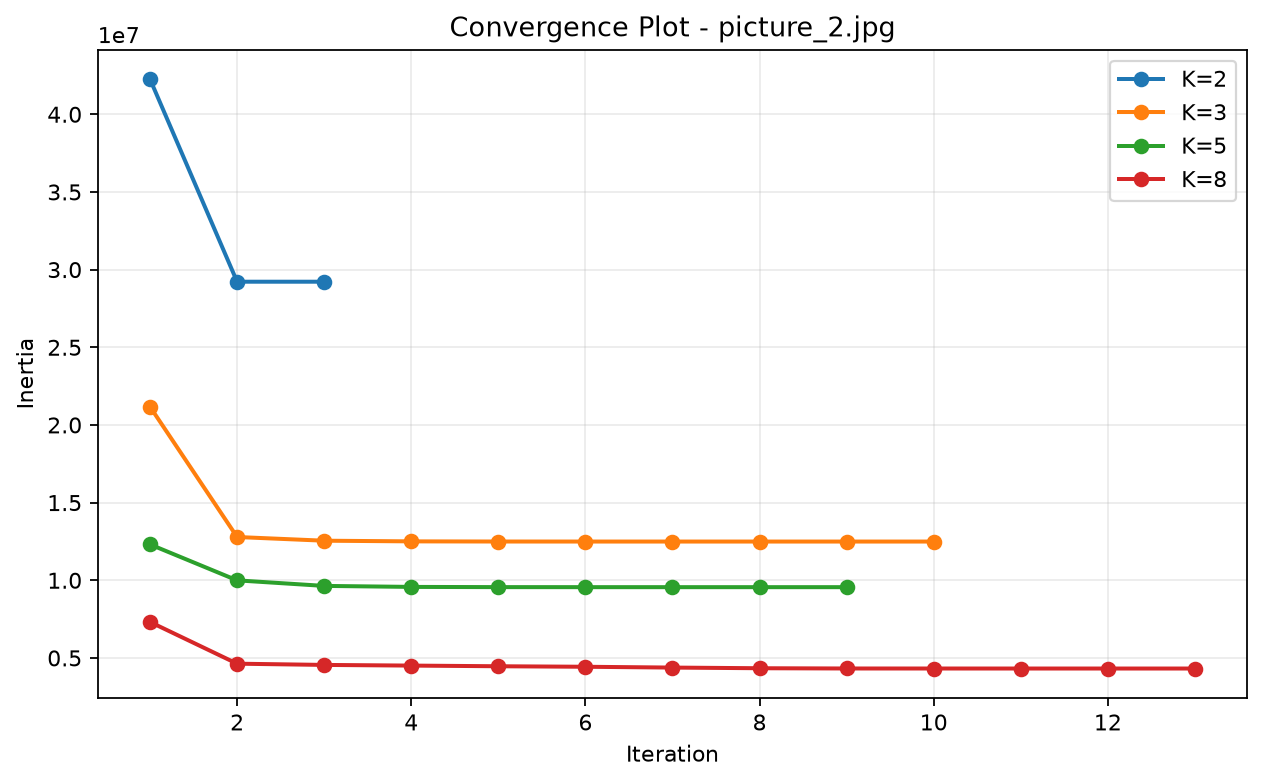
\includegraphics[width=\textwidth]{figures/lab31/convergence_plot_picture_2.png}
  \caption{Convergence: Picture 2}
\end{figure}
\begin{figure}[H]
  \centering
  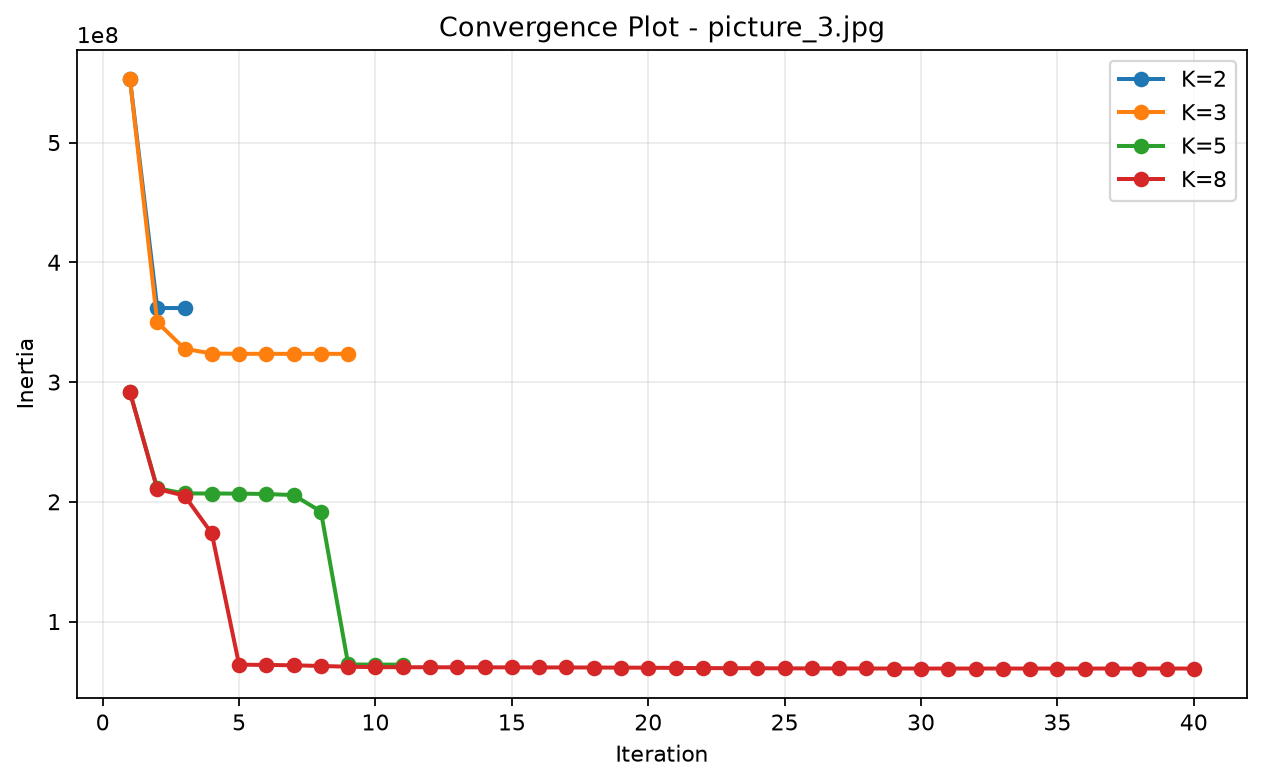
\includegraphics[width=\textwidth]{figures/lab31/convergence_plot_picture_3.png}
  \caption{Convergence: Picture 3}
\end{figure}
\begin{figure}[H]
  \centering
  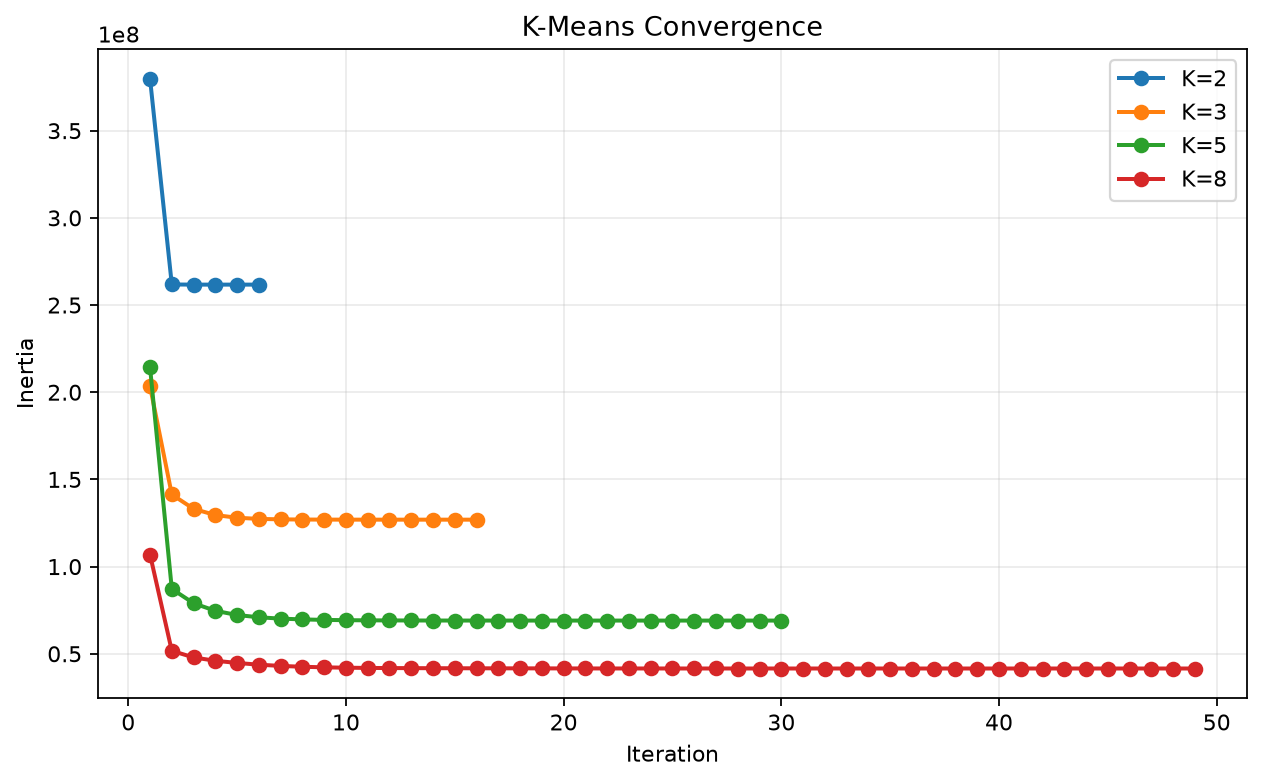
\includegraphics[width=\textwidth]{figures/lab31/convergence_plot.png}
  \caption{Convergence: all pictures}
\end{figure}
\begin{figure}[H]
  \centering
  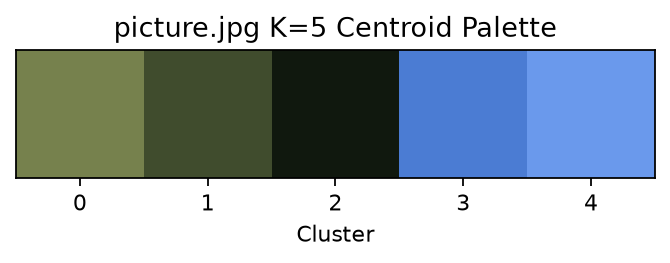
\includegraphics[width=\textwidth]{figures/lab31/color_palette_picture_k5.png}
  \caption{Color palette at K=5}
\end{figure}
\end{figure}

\begin{figure}[H]\centering
\begin{figure}[H]
  \centering
  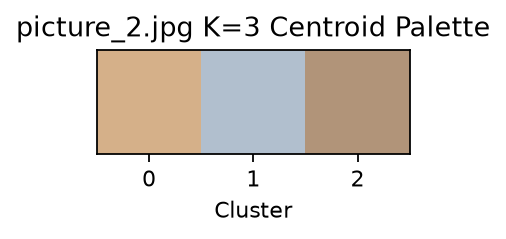
\includegraphics[width=\textwidth]{figures/lab31/color_palette_picture_2_k3.png}
  \caption{Palette: Picture 2, K=3}
\end{figure}
\begin{figure}[H]
  \centering
  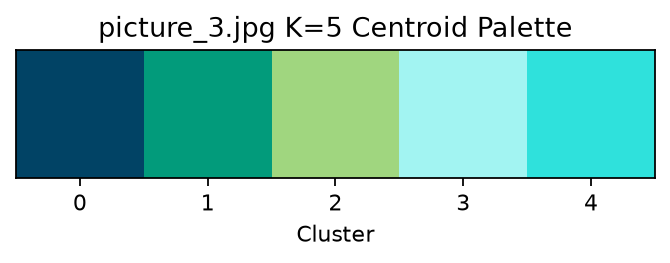
\includegraphics[width=\textwidth]{figures/lab31/color_palette_picture_3_k5.png}
  \caption{Palette: Picture 3, K=5}
\end{figure}
\begin{figure}[H]
  \centering
  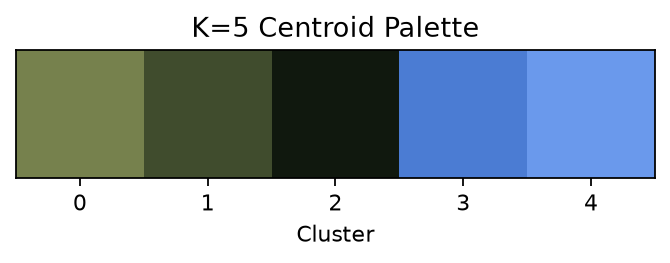
\includegraphics[width=\textwidth]{figures/lab31/color_palette_k5.png}
  \caption{Color palette K=5 detail}
\end{figure}
\end{figure}

\begin{notebox}
\textbf{Always use silhouette alongside elbow for choosing K.} Inertia is guaranteed to decrease with more clusters — it can never penalize over-segmentation. Silhouette penalizes fragmented clusters by detecting overlap: for the primary image, the drop from 0.518 (K=5) to 0.492 (K=8) is the critical signal to stop. The convergence plot shows monotonic descent for all K, confirming healthy optimization with no oscillation or divergence. K=5 is selected because (a) the elbow flattens after this point with marginal inertia reduction of only 39.813\% across three additional clusters, (b) silhouette remains above the 0.500 threshold, and (c) the 30 iterations required to converge are computationally acceptable for the 91{,}700-pixel dataset.
\end{notebox}
